\documentclass[1p]{elsarticle_modified}
%\bibliographystyle{elsarticle-num}

%\usepackage[colorlinks]{hyperref}
%\usepackage{abbrmath_seonhwa} %\Abb, \Ascr, \Acal ,\Abf, \Afrak
\usepackage{amsfonts}
\usepackage{amssymb}
\usepackage{amsmath}
\usepackage{amsthm}
\usepackage{scalefnt}
\usepackage{amsbsy}
\usepackage{kotex}
\usepackage{caption}
\usepackage{subfig}
\usepackage{color}
\usepackage{graphicx}
\usepackage{xcolor} %% white, black, red, green, blue, cyan, magenta, yellow
\usepackage{float}
\usepackage{setspace}
\usepackage{hyperref}

\usepackage{tikz}
\usetikzlibrary{arrows}

\usepackage{multirow}
\usepackage{array} % fixed length table
\usepackage{hhline}

%%%%%%%%%%%%%%%%%%%%%
\makeatletter
\renewcommand*\env@matrix[1][\arraystretch]{%
	\edef\arraystretch{#1}%
	\hskip -\arraycolsep
	\let\@ifnextchar\new@ifnextchar
	\array{*\c@MaxMatrixCols c}}
\makeatother %https://tex.stackexchange.com/questions/14071/how-can-i-increase-the-line-spacing-in-a-matrix
%%%%%%%%%%%%%%%

\usepackage[normalem]{ulem}

\newcommand{\msout}[1]{\ifmmode\text{\sout{\ensuremath{#1}}}\else\sout{#1}\fi}
%SOURCE: \msout is \stkout macro in https://tex.stackexchange.com/questions/20609/strikeout-in-math-mode

\newcommand{\cancel}[1]{
	\ifmmode
	{\color{red}\msout{#1}}
	\else
	{\color{red}\sout{#1}}
	\fi
}

\newcommand{\add}[1]{
	{\color{blue}\uwave{#1}}
}

\newcommand{\replace}[2]{
	\ifmmode
	{\color{red}\msout{#1}}{\color{blue}\uwave{#2}}
	\else
	{\color{red}\sout{#1}}{\color{blue}\uwave{#2}}
	\fi
}

\newcommand{\Sol}{\mathcal{S}} %segment
\newcommand{\D}{D} %diagram
\newcommand{\A}{\mathcal{A}} %arc


%%%%%%%%%%%%%%%%%%%%%%%%%%%%%5 test

\def\sl{\operatorname{\textup{SL}}(2,\Cbb)}
\def\psl{\operatorname{\textup{PSL}}(2,\Cbb)}
\def\quan{\mkern 1mu \triangleright \mkern 1mu}

\theoremstyle{definition}
\newtheorem{thm}{Theorem}[section]
\newtheorem{prop}[thm]{Proposition}
\newtheorem{lem}[thm]{Lemma}
\newtheorem{ques}[thm]{Question}
\newtheorem{cor}[thm]{Corollary}
\newtheorem{defn}[thm]{Definition}
\newtheorem{exam}[thm]{Example}
\newtheorem{rmk}[thm]{Remark}
\newtheorem{alg}[thm]{Algorithm}

\newcommand{\I}{\sqrt{-1}}
\begin{document}

%\begin{frontmatter}
%
%\title{Boundary parabolic representations of knots up to 8 crossings}
%
%%% Group authors per affiliation:
%\author{Yunhi Cho} 
%\address{Department of Mathematics, University of Seoul, Seoul, Korea}
%\ead{yhcho@uos.ac.kr}
%
%
%\author{Seonhwa Kim} %\fnref{s_kim}}
%\address{Center for Geometry and Physics, Institute for Basic Science, Pohang, 37673, Korea}
%\ead{ryeona17@ibs.re.kr}
%
%\author{Hyuk Kim}
%\address{Department of Mathematical Sciences, Seoul National University, Seoul 08826, Korea}
%\ead{hyukkim@snu.ac.kr}
%
%\author{Seokbeom Yoon}
%\address{Department of Mathematical Sciences, Seoul National University, Seoul, 08826,  Korea}
%\ead{sbyoon15@snu.ac.kr}
%
%\begin{abstract}
%We find all boundary parabolic representation of knots up to 8 crossings.
%
%\end{abstract}
%\begin{keyword}
%    \MSC[2010] 57M25 
%\end{keyword}
%
%\end{frontmatter}

%\linenumbers
%\tableofcontents
%
\newcommand\colored[1]{\textcolor{white}{\rule[-0.35ex]{0.8em}{1.4ex}}\kern-0.8em\color{red} #1}%
%\newcommand\colored[1]{\textcolor{white}{ #1}\kern-2.17ex	\textcolor{white}{ #1}\kern-1.81ex	\textcolor{white}{ #1}\kern-2.15ex\color{red}#1	}

{\Large $\underline{12a_{0361}~(K12a_{0361})}$}

\setlength{\tabcolsep}{10pt}
\renewcommand{\arraystretch}{1.6}
\vspace{1cm}\begin{tabular}{m{100pt}>{\centering\arraybackslash}m{274pt}}
\multirow{5}{120pt}{
	\centering
	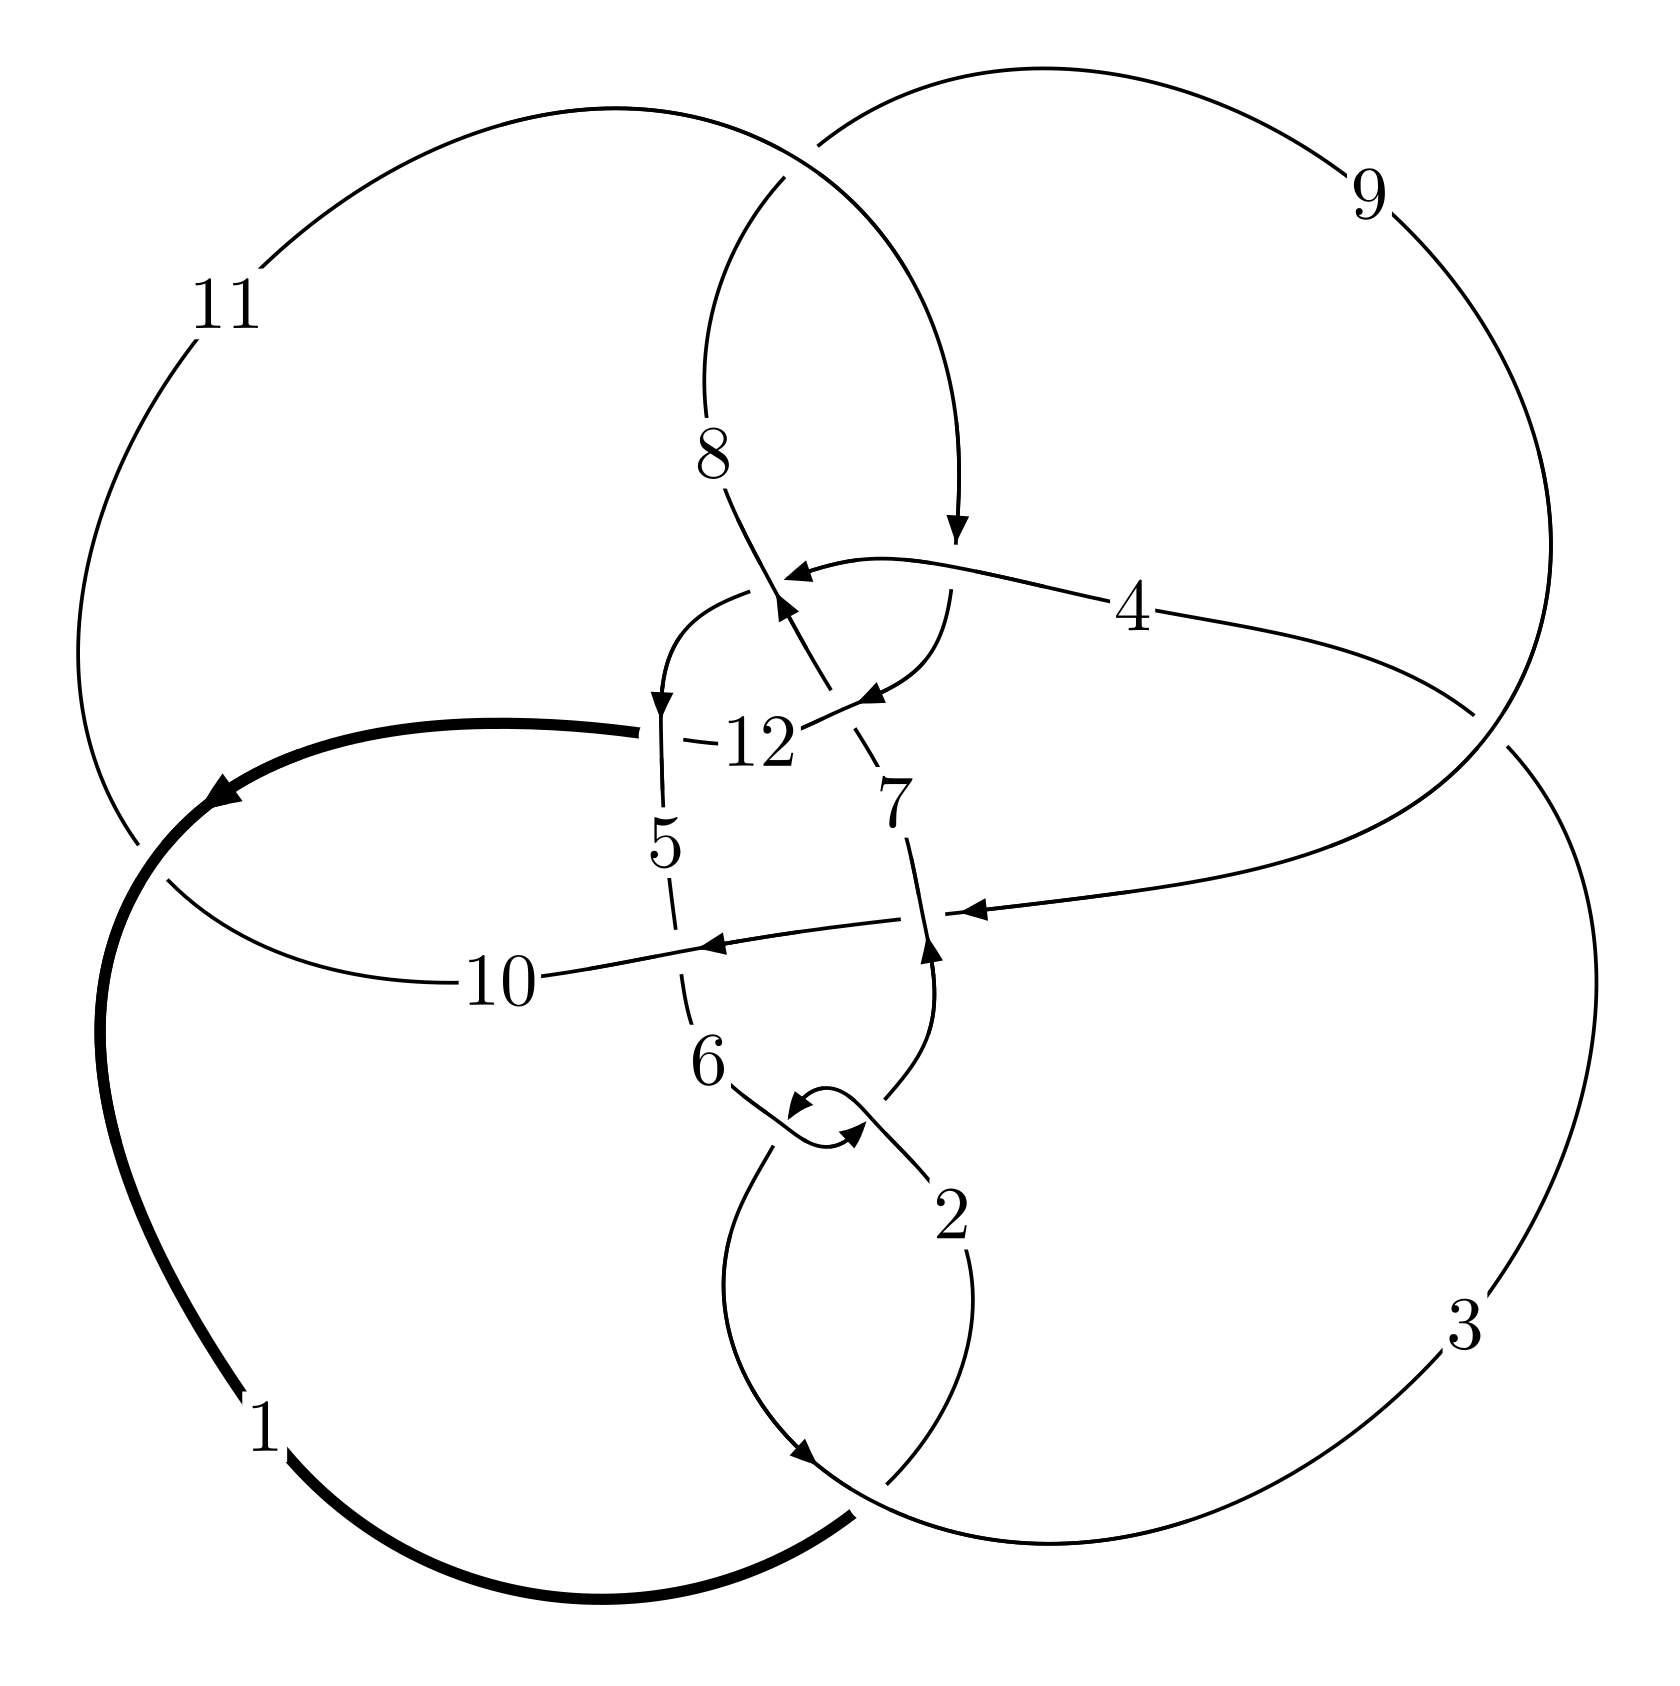
\includegraphics[width=112pt]{../../../GIT/diagram.site/Diagrams/png/1162_12a_0361.png}\\
\ \ \ A knot diagram\footnotemark}&
\allowdisplaybreaks
\textbf{Linearized knot diagam} \\
\cline{2-2}
 &
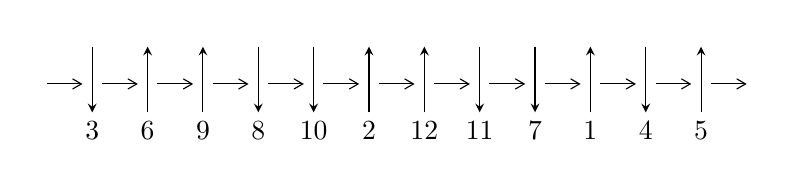
\begin{tikzpicture}[x=20pt, y=17pt]
	% nodes
	\node (C0) at (0, 0) {};
	\node (C1) at (1, 0) {};
	\node (C1U) at (1, +1) {};
	\node (C1D) at (1, -1) {3};

	\node (C2) at (2, 0) {};
	\node (C2U) at (2, +1) {};
	\node (C2D) at (2, -1) {6};

	\node (C3) at (3, 0) {};
	\node (C3U) at (3, +1) {};
	\node (C3D) at (3, -1) {9};

	\node (C4) at (4, 0) {};
	\node (C4U) at (4, +1) {};
	\node (C4D) at (4, -1) {8};

	\node (C5) at (5, 0) {};
	\node (C5U) at (5, +1) {};
	\node (C5D) at (5, -1) {10};

	\node (C6) at (6, 0) {};
	\node (C6U) at (6, +1) {};
	\node (C6D) at (6, -1) {2};

	\node (C7) at (7, 0) {};
	\node (C7U) at (7, +1) {};
	\node (C7D) at (7, -1) {12};

	\node (C8) at (8, 0) {};
	\node (C8U) at (8, +1) {};
	\node (C8D) at (8, -1) {11};

	\node (C9) at (9, 0) {};
	\node (C9U) at (9, +1) {};
	\node (C9D) at (9, -1) {7};

	\node (C10) at (10, 0) {};
	\node (C10U) at (10, +1) {};
	\node (C10D) at (10, -1) {1};

	\node (C11) at (11, 0) {};
	\node (C11U) at (11, +1) {};
	\node (C11D) at (11, -1) {4};

	\node (C12) at (12, 0) {};
	\node (C12U) at (12, +1) {};
	\node (C12D) at (12, -1) {5};
	\node (C13) at (13, 0) {};

	% arrows
	\draw[->,>={angle 60}]
	(C0) edge (C1) (C1) edge (C2) (C2) edge (C3) (C3) edge (C4) (C4) edge (C5) (C5) edge (C6) (C6) edge (C7) (C7) edge (C8) (C8) edge (C9) (C9) edge (C10) (C10) edge (C11) (C11) edge (C12) (C12) edge (C13) ;	\draw[->,>=stealth]
	(C1U) edge (C1D) (C2D) edge (C2U) (C3D) edge (C3U) (C4U) edge (C4D) (C5U) edge (C5D) (C6D) edge (C6U) (C7D) edge (C7U) (C8U) edge (C8D) (C9U) edge (C9D) (C10D) edge (C10U) (C11U) edge (C11D) (C12D) edge (C12U) ;
	\end{tikzpicture} \\
\hhline{~~} \\& 
\textbf{Solving Sequence} \\ \cline{2-2} 
 &
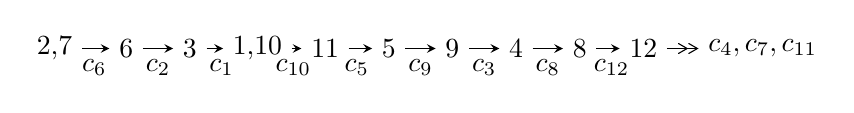
\begin{tikzpicture}[x=23pt, y=7pt]
	% node
	\node (A0) at (-1/8, 0) {2,7};
	\node (A1) at (1, 0) {6};
	\node (A2) at (2, 0) {3};
	\node (A3) at (49/16, 0) {1,10};
	\node (A4) at (33/8, 0) {11};
	\node (A5) at (41/8, 0) {5};
	\node (A6) at (49/8, 0) {9};
	\node (A7) at (57/8, 0) {4};
	\node (A8) at (65/8, 0) {8};
	\node (A9) at (73/8, 0) {12};
	\node (C1) at (1/2, -1) {$c_{6}$};
	\node (C2) at (3/2, -1) {$c_{2}$};
	\node (C3) at (5/2, -1) {$c_{1}$};
	\node (C4) at (29/8, -1) {$c_{10}$};
	\node (C5) at (37/8, -1) {$c_{5}$};
	\node (C6) at (45/8, -1) {$c_{9}$};
	\node (C7) at (53/8, -1) {$c_{3}$};
	\node (C8) at (61/8, -1) {$c_{8}$};
	\node (C9) at (69/8, -1) {$c_{12}$};
	\node (A10) at (11, 0) {$c_{4},c_{7},c_{11}$};

	% edge
	\draw[->,>=stealth]	
	(A0) edge (A1) (A1) edge (A2) (A2) edge (A3) (A3) edge (A4) (A4) edge (A5) (A5) edge (A6) (A6) edge (A7) (A7) edge (A8) (A8) edge (A9) ;
	\draw[->>,>={angle 60}]	
	(A9) edge (A10);
\end{tikzpicture} \\ 

\end{tabular} \\

\footnotetext{
The image of knot diagram is generated by the software ``\textbf{Draw programme}" developed by Andrew Bartholomew(\url{http://www.layer8.co.uk/maths/draw/index.htm\#Running-draw}), where we modified some parts for our purpose(\url{https://github.com/CATsTAILs/LinksPainter}).
}\phantom \\ \newline 
\centering \textbf{Ideals for irreducible components\footnotemark of $X_{\text{par}}$} 
 
\begin{align*}
I^u_{1}&=\langle 
-5.19484\times10^{727} u^{208}+8.25909\times10^{726} u^{207}+\cdots+2.89794\times10^{726} b-5.95025\times10^{728},\\
\phantom{I^u_{1}}&\phantom{= \langle  }-5.74402\times10^{728} u^{208}-2.50115\times10^{729} u^{207}+\cdots+8.98362\times10^{727} a+8.40848\times10^{730},\\
\phantom{I^u_{1}}&\phantom{= \langle  }u^{209}+u^{208}+\cdots+157 u-31\rangle \\
I^u_{2}&=\langle 
-5.62203\times10^{24} u^{44}-2.14255\times10^{24} u^{43}+\cdots+1.91127\times10^{24} b-4.18208\times10^{24},\\
\phantom{I^u_{2}}&\phantom{= \langle  }1.38584\times10^{25} u^{44}-7.72588\times10^{23} u^{43}+\cdots+1.91127\times10^{24} a-1.67886\times10^{25},\;u^{45}+13 u^{43}+\cdots+3 u+1\rangle \\
\\
\end{align*}
\raggedright * 2 irreducible components of $\dim_{\mathbb{C}}=0$, with total 254 representations.\\
\footnotetext{All coefficients of polynomials are rational numbers. But the coefficients are sometimes approximated in decimal forms when there is not enough margin.}
\newpage
\renewcommand{\arraystretch}{1}
\centering \section*{I. $I^u_{1}= \langle -5.19\times10^{727} u^{208}+8.26\times10^{726} u^{207}+\cdots+2.90\times10^{726} b-5.95\times10^{728},\;-5.74\times10^{728} u^{208}-2.50\times10^{729} u^{207}+\cdots+8.98\times10^{727} a+8.41\times10^{730},\;u^{209}+u^{208}+\cdots+157 u-31 \rangle$}
\flushleft \textbf{(i) Arc colorings}\\
\begin{tabular}{m{7pt} m{180pt} m{7pt} m{180pt} }
\flushright $a_{2}=$&$\begin{pmatrix}0\\u\end{pmatrix}$ \\
\flushright $a_{7}=$&$\begin{pmatrix}1\\0\end{pmatrix}$ \\
\flushright $a_{6}=$&$\begin{pmatrix}1\\u^2\end{pmatrix}$ \\
\flushright $a_{3}=$&$\begin{pmatrix}u\\u^3+u\end{pmatrix}$ \\
\flushright $a_{1}=$&$\begin{pmatrix}u^3\\u^5+u^3+u\end{pmatrix}$ \\
\flushright $a_{10}=$&$\begin{pmatrix}6.39389 u^{208}+27.8413 u^{207}+\cdots+5326.95 u-935.980\\17.9260 u^{208}-2.84999 u^{207}+\cdots-1746.62 u+205.327\end{pmatrix}$ \\
\flushright $a_{11}=$&$\begin{pmatrix}24.0595 u^{208}+43.1655 u^{207}+\cdots+7005.92 u-1310.55\\11.9868 u^{208}-6.46156 u^{207}+\cdots-2018.72 u+284.552\end{pmatrix}$ \\
\flushright $a_{5}=$&$\begin{pmatrix}47.9537 u^{208}+46.5295 u^{207}+\cdots+6025.57 u-1293.15\\-9.59584 u^{208}-6.09771 u^{207}+\cdots-555.561 u+146.161\end{pmatrix}$ \\
\flushright $a_{9}=$&$\begin{pmatrix}24.3199 u^{208}+24.9913 u^{207}+\cdots+3580.32 u-730.653\\17.9260 u^{208}-2.84999 u^{207}+\cdots-1746.62 u+205.327\end{pmatrix}$ \\
\flushright $a_{4}=$&$\begin{pmatrix}-32.6099 u^{208}-30.8544 u^{207}+\cdots-3776.28 u+834.973\\15.2112 u^{208}+11.6311 u^{207}+\cdots+1168.81 u-280.462\end{pmatrix}$ \\
\flushright $a_{8}=$&$\begin{pmatrix}36.5951 u^{208}-2.85855 u^{207}+\cdots-2738.98 u+271.752\\-3.36340 u^{208}-5.69928 u^{207}+\cdots-666.592 u+129.498\end{pmatrix}$ \\
\flushright $a_{12}=$&$\begin{pmatrix}35.2543 u^{208}+47.3291 u^{207}+\cdots+6049.61 u-1248.70\\4.43078 u^{208}+6.47752 u^{207}+\cdots+921.918 u-175.511\end{pmatrix}$\\&\end{tabular}
\flushleft \textbf{(ii) Obstruction class $= -1$}\\~\\
\flushleft \textbf{(iii) Cusp Shapes $= -1268.80 u^{208}-749.344 u^{207}+\cdots-65537.2 u+17961.7$}\\~\\
\newpage\renewcommand{\arraystretch}{1}
\flushleft \textbf{(iv) u-Polynomials at the component}\newline \\
\begin{tabular}{m{50pt}|m{274pt}}
Crossings & \hspace{64pt}u-Polynomials at each crossing \\
\hline $$\begin{aligned}c_{1}\end{aligned}$$&$\begin{aligned}
&u^{209}+95 u^{208}+\cdots-21355 u-961
\end{aligned}$\\
\hline $$\begin{aligned}c_{2},c_{6}\end{aligned}$$&$\begin{aligned}
&u^{209}- u^{208}+\cdots+157 u+31
\end{aligned}$\\
\hline $$\begin{aligned}c_{3}\end{aligned}$$&$\begin{aligned}
&u^{209}+u^{208}+\cdots+10419082 u+304643
\end{aligned}$\\
\hline $$\begin{aligned}c_{4}\end{aligned}$$&$\begin{aligned}
&u^{209}+6 u^{208}+\cdots-116 u+8
\end{aligned}$\\
\hline $$\begin{aligned}c_{5}\end{aligned}$$&$\begin{aligned}
&u^{209}- u^{208}+\cdots+2641791 u+518269
\end{aligned}$\\
\hline $$\begin{aligned}c_{7}\end{aligned}$$&$\begin{aligned}
&u^{209}+3 u^{208}+\cdots+41 u+1
\end{aligned}$\\
\hline $$\begin{aligned}c_{8}\end{aligned}$$&$\begin{aligned}
&u^{209}+10 u^{208}+\cdots-360 u+13
\end{aligned}$\\
\hline $$\begin{aligned}c_{9}\end{aligned}$$&$\begin{aligned}
&u^{209}+5 u^{208}+\cdots+23494787 u+2058527
\end{aligned}$\\
\hline $$\begin{aligned}c_{10}\end{aligned}$$&$\begin{aligned}
&u^{209}-5 u^{208}+\cdots+23728 u+1856
\end{aligned}$\\
\hline $$\begin{aligned}c_{11}\end{aligned}$$&$\begin{aligned}
&u^{209}+4 u^{208}+\cdots+71 u-173
\end{aligned}$\\
\hline $$\begin{aligned}c_{12}\end{aligned}$$&$\begin{aligned}
&u^{209}+3 u^{208}+\cdots+132 u+1
\end{aligned}$\\
\hline
\end{tabular}\\~\\
\newpage\renewcommand{\arraystretch}{1}
\flushleft \textbf{(v) Riley Polynomials at the component}\newline \\
\begin{tabular}{m{50pt}|m{274pt}}
Crossings & \hspace{64pt}Riley Polynomials at each crossing \\
\hline $$\begin{aligned}c_{1}\end{aligned}$$&$\begin{aligned}
&y^{209}+55 y^{208}+\cdots+62744853 y-923521
\end{aligned}$\\
\hline $$\begin{aligned}c_{2},c_{6}\end{aligned}$$&$\begin{aligned}
&y^{209}+95 y^{208}+\cdots-21355 y-961
\end{aligned}$\\
\hline $$\begin{aligned}c_{3}\end{aligned}$$&$\begin{aligned}
&y^{209}+47 y^{208}+\cdots-7664051227998 y-92807357449
\end{aligned}$\\
\hline $$\begin{aligned}c_{4}\end{aligned}$$&$\begin{aligned}
&y^{209}+28 y^{208}+\cdots-2608 y-64
\end{aligned}$\\
\hline $$\begin{aligned}c_{5}\end{aligned}$$&$\begin{aligned}
&y^{209}+29 y^{208}+\cdots-14754978917513 y-268602756361
\end{aligned}$\\
\hline $$\begin{aligned}c_{7}\end{aligned}$$&$\begin{aligned}
&y^{209}-13 y^{208}+\cdots+169 y-1
\end{aligned}$\\
\hline $$\begin{aligned}c_{8}\end{aligned}$$&$\begin{aligned}
&y^{209}-14 y^{208}+\cdots-67974 y-169
\end{aligned}$\\
\hline $$\begin{aligned}c_{9}\end{aligned}$$&$\begin{aligned}
&y^{209}+y^{208}+\cdots-123218028405125 y-4237533409729
\end{aligned}$\\
\hline $$\begin{aligned}c_{10}\end{aligned}$$&$\begin{aligned}
&y^{209}-37 y^{208}+\cdots+94845696 y-3444736
\end{aligned}$\\
\hline $$\begin{aligned}c_{11}\end{aligned}$$&$\begin{aligned}
&y^{209}-2 y^{208}+\cdots+2076543 y-29929
\end{aligned}$\\
\hline $$\begin{aligned}c_{12}\end{aligned}$$&$\begin{aligned}
&y^{209}-41 y^{208}+\cdots+5070 y-1
\end{aligned}$\\
\hline
\end{tabular}\\~\\
\newpage\flushleft \textbf{(vi) Complex Volumes and Cusp Shapes}
$$\begin{array}{c|c|c}  
\text{Solutions to }I^u_{1}& \I (\text{vol} + \sqrt{-1}CS) & \text{Cusp shape}\\
 \hline 
\begin{aligned}
u &= -0.414459 + 0.912946 I \\
a &= -0.003703 + 1.328120 I \\
b &= \phantom{-}0.055954 + 0.726607 I\end{aligned}
 & -0.797811 + 0.322751 I & \phantom{-0.000000 } 0 \\ \hline\begin{aligned}
u &= -0.414459 - 0.912946 I \\
a &= -0.003703 - 1.328120 I \\
b &= \phantom{-}0.055954 - 0.726607 I\end{aligned}
 & -0.797811 - 0.322751 I & \phantom{-0.000000 } 0 \\ \hline\begin{aligned}
u &= \phantom{-}0.789395 + 0.604559 I \\
a &= -0.382992 + 0.377656 I \\
b &= \phantom{-}0.426451 + 1.127850 I\end{aligned}
 & \phantom{-}5.55730 - 7.04279 I & \phantom{-0.000000 } 0 \\ \hline\begin{aligned}
u &= \phantom{-}0.789395 - 0.604559 I \\
a &= -0.382992 - 0.377656 I \\
b &= \phantom{-}0.426451 - 1.127850 I\end{aligned}
 & \phantom{-}5.55730 + 7.04279 I & \phantom{-0.000000 } 0 \\ \hline\begin{aligned}
u &= \phantom{-}0.888897 + 0.443556 I \\
a &= \phantom{-}0.138371 + 0.096590 I \\
b &= \phantom{-}0.90624 + 1.40713 I\end{aligned}
 & \phantom{-}1.34487 - 7.80456 I & \phantom{-0.000000 } 0 \\ \hline\begin{aligned}
u &= \phantom{-}0.888897 - 0.443556 I \\
a &= \phantom{-}0.138371 - 0.096590 I \\
b &= \phantom{-}0.90624 - 1.40713 I\end{aligned}
 & \phantom{-}1.34487 + 7.80456 I & \phantom{-0.000000 } 0 \\ \hline\begin{aligned}
u &= \phantom{-}0.522878 + 0.844028 I \\
a &= -2.51795 - 0.11586 I \\
b &= \phantom{-}0.56972 - 1.52968 I\end{aligned}
 & \phantom{-}2.55861 + 5.83117 I & \phantom{-0.000000 } 0 \\ \hline\begin{aligned}
u &= \phantom{-}0.522878 - 0.844028 I \\
a &= -2.51795 + 0.11586 I \\
b &= \phantom{-}0.56972 + 1.52968 I\end{aligned}
 & \phantom{-}2.55861 - 5.83117 I & \phantom{-0.000000 } 0 \\ \hline\begin{aligned}
u &= \phantom{-}0.509684 + 0.869877 I \\
a &= \phantom{-}0.924253 - 0.199476 I \\
b &= \phantom{-}0.29260 + 1.86459 I\end{aligned}
 & \phantom{-}2.48549 - 1.65200 I & \phantom{-0.000000 } 0 \\ \hline\begin{aligned}
u &= \phantom{-}0.509684 - 0.869877 I \\
a &= \phantom{-}0.924253 + 0.199476 I \\
b &= \phantom{-}0.29260 - 1.86459 I\end{aligned}
 & \phantom{-}2.48549 + 1.65200 I & \phantom{-0.000000 } 0\\
 \hline 
 \end{array}$$\newpage$$\begin{array}{c|c|c}  
\text{Solutions to }I^u_{1}& \I (\text{vol} + \sqrt{-1}CS) & \text{Cusp shape}\\
 \hline 
\begin{aligned}
u &= \phantom{-}0.288077 + 0.946097 I \\
a &= -0.77080 - 1.25654 I \\
b &= \phantom{-}1.27234 + 0.80753 I\end{aligned}
 & -3.69355 - 0.54833 I & \phantom{-0.000000 } 0 \\ \hline\begin{aligned}
u &= \phantom{-}0.288077 - 0.946097 I \\
a &= -0.77080 + 1.25654 I \\
b &= \phantom{-}1.27234 - 0.80753 I\end{aligned}
 & -3.69355 + 0.54833 I & \phantom{-0.000000 } 0 \\ \hline\begin{aligned}
u &= -0.688092 + 0.708394 I \\
a &= -0.96931 - 1.05574 I \\
b &= -1.22304 + 1.67861 I\end{aligned}
 & \phantom{-}2.45193 + 6.07675 I & \phantom{-0.000000 } 0 \\ \hline\begin{aligned}
u &= -0.688092 - 0.708394 I \\
a &= -0.96931 + 1.05574 I \\
b &= -1.22304 - 1.67861 I\end{aligned}
 & \phantom{-}2.45193 - 6.07675 I & \phantom{-0.000000 } 0 \\ \hline\begin{aligned}
u &= \phantom{-}0.776949 + 0.608508 I \\
a &= \phantom{-}0.631967 + 0.150693 I \\
b &= -0.369573 - 0.528778 I\end{aligned}
 & \phantom{-}4.29894 - 1.79618 I & \phantom{-0.000000 } 0 \\ \hline\begin{aligned}
u &= \phantom{-}0.776949 - 0.608508 I \\
a &= \phantom{-}0.631967 - 0.150693 I \\
b &= -0.369573 + 0.528778 I\end{aligned}
 & \phantom{-}4.29894 + 1.79618 I & \phantom{-0.000000 } 0 \\ \hline\begin{aligned}
u &= -0.933186 + 0.395299 I \\
a &= \phantom{-}0.036618 + 0.138293 I \\
b &= \phantom{-}0.674525 - 1.168200 I\end{aligned}
 & \phantom{-}3.82194 + 6.78600 I & \phantom{-0.000000 } 0 \\ \hline\begin{aligned}
u &= -0.933186 - 0.395299 I \\
a &= \phantom{-}0.036618 - 0.138293 I \\
b &= \phantom{-}0.674525 + 1.168200 I\end{aligned}
 & \phantom{-}3.82194 - 6.78600 I & \phantom{-0.000000 } 0 \\ \hline\begin{aligned}
u &= \phantom{-}0.324625 + 0.960718 I \\
a &= \phantom{-}2.27632 + 0.63428 I \\
b &= -1.170670 - 0.467528 I\end{aligned}
 & -2.71146 - 6.61718 I & \phantom{-0.000000 } 0 \\ \hline\begin{aligned}
u &= \phantom{-}0.324625 - 0.960718 I \\
a &= \phantom{-}2.27632 - 0.63428 I \\
b &= -1.170670 + 0.467528 I\end{aligned}
 & -2.71146 + 6.61718 I & \phantom{-0.000000 } 0\\
 \hline 
 \end{array}$$\newpage$$\begin{array}{c|c|c}  
\text{Solutions to }I^u_{1}& \I (\text{vol} + \sqrt{-1}CS) & \text{Cusp shape}\\
 \hline 
\begin{aligned}
u &= -0.335784 + 0.958593 I \\
a &= \phantom{-}1.96499 + 0.06488 I \\
b &= -0.495656 - 0.383507 I\end{aligned}
 & -0.63720 - 3.37626 I & \phantom{-0.000000 } 0 \\ \hline\begin{aligned}
u &= -0.335784 - 0.958593 I \\
a &= \phantom{-}1.96499 - 0.06488 I \\
b &= -0.495656 + 0.383507 I\end{aligned}
 & -0.63720 + 3.37626 I & \phantom{-0.000000 } 0 \\ \hline\begin{aligned}
u &= \phantom{-}0.906499 + 0.467616 I \\
a &= \phantom{-}0.101936 + 0.117894 I \\
b &= -0.828780 - 1.041650 I\end{aligned}
 & \phantom{-}3.89808 - 7.70135 I & \phantom{-0.000000 } 0 \\ \hline\begin{aligned}
u &= \phantom{-}0.906499 - 0.467616 I \\
a &= \phantom{-}0.101936 - 0.117894 I \\
b &= -0.828780 + 1.041650 I\end{aligned}
 & \phantom{-}3.89808 + 7.70135 I & \phantom{-0.000000 } 0 \\ \hline\begin{aligned}
u &= -0.920973 + 0.441679 I \\
a &= -0.0746547 - 0.0361478 I \\
b &= -0.96410 + 1.31177 I\end{aligned}
 & \phantom{-}2.7171 + 16.3636 I & \phantom{-0.000000 } 0 \\ \hline\begin{aligned}
u &= -0.920973 - 0.441679 I \\
a &= -0.0746547 + 0.0361478 I \\
b &= -0.96410 - 1.31177 I\end{aligned}
 & \phantom{-}2.7171 - 16.3636 I & \phantom{-0.000000 } 0 \\ \hline\begin{aligned}
u &= -0.431563 + 0.876562 I \\
a &= -3.20089 - 1.16991 I \\
b &= \phantom{-}1.047510 - 0.091862 I\end{aligned}
 & -1.94953 - 1.79271 I & \phantom{-0.000000 } 0 \\ \hline\begin{aligned}
u &= -0.431563 - 0.876562 I \\
a &= -3.20089 + 1.16991 I \\
b &= \phantom{-}1.047510 + 0.091862 I\end{aligned}
 & -1.94953 + 1.79271 I & \phantom{-0.000000 } 0 \\ \hline\begin{aligned}
u &= \phantom{-}0.305606 + 0.978245 I \\
a &= \phantom{-}0.709704 - 0.806685 I \\
b &= \phantom{-}0.47503 + 1.33783 I\end{aligned}
 & -3.90365 - 0.86232 I & \phantom{-0.000000 } 0 \\ \hline\begin{aligned}
u &= \phantom{-}0.305606 - 0.978245 I \\
a &= \phantom{-}0.709704 + 0.806685 I \\
b &= \phantom{-}0.47503 - 1.33783 I\end{aligned}
 & -3.90365 + 0.86232 I & \phantom{-0.000000 } 0\\
 \hline 
 \end{array}$$\newpage$$\begin{array}{c|c|c}  
\text{Solutions to }I^u_{1}& \I (\text{vol} + \sqrt{-1}CS) & \text{Cusp shape}\\
 \hline 
\begin{aligned}
u &= \phantom{-}0.537969 + 0.876020 I \\
a &= -0.111044 + 0.845335 I \\
b &= -0.65330 - 1.46273 I\end{aligned}
 & \phantom{-}2.58623 + 5.57819 I & \phantom{-0.000000 } 0 \\ \hline\begin{aligned}
u &= \phantom{-}0.537969 - 0.876020 I \\
a &= -0.111044 - 0.845335 I \\
b &= -0.65330 + 1.46273 I\end{aligned}
 & \phantom{-}2.58623 - 5.57819 I & \phantom{-0.000000 } 0 \\ \hline\begin{aligned}
u &= -0.422248 + 0.941029 I \\
a &= -1.93427 + 1.91849 I \\
b &= \phantom{-}1.76946 - 0.47172 I\end{aligned}
 & -3.11518 - 2.10460 I & \phantom{-0.000000 } 0 \\ \hline\begin{aligned}
u &= -0.422248 - 0.941029 I \\
a &= -1.93427 - 1.91849 I \\
b &= \phantom{-}1.76946 + 0.47172 I\end{aligned}
 & -3.11518 + 2.10460 I & \phantom{-0.000000 } 0 \\ \hline\begin{aligned}
u &= -0.893300 + 0.373250 I \\
a &= \phantom{-}0.011105 - 0.233458 I \\
b &= -0.711696 + 0.565707 I\end{aligned}
 & -1.58574 - 1.28213 I & \phantom{-0.000000 } 0 \\ \hline\begin{aligned}
u &= -0.893300 - 0.373250 I \\
a &= \phantom{-}0.011105 + 0.233458 I \\
b &= -0.711696 - 0.565707 I\end{aligned}
 & -1.58574 + 1.28213 I & \phantom{-0.000000 } 0 \\ \hline\begin{aligned}
u &= \phantom{-}0.556619 + 0.778290 I \\
a &= \phantom{-}1.77329 + 0.45235 I \\
b &= -0.919267 + 0.824154 I\end{aligned}
 & \phantom{-}2.85872 - 1.14050 I & \phantom{-0.000000 } 0 \\ \hline\begin{aligned}
u &= \phantom{-}0.556619 - 0.778290 I \\
a &= \phantom{-}1.77329 - 0.45235 I \\
b &= -0.919267 - 0.824154 I\end{aligned}
 & \phantom{-}2.85872 + 1.14050 I & \phantom{-0.000000 } 0 \\ \hline\begin{aligned}
u &= -0.411300 + 0.958728 I \\
a &= \phantom{-}1.80933 - 0.17952 I \\
b &= -0.626405 + 0.192231 I\end{aligned}
 & -0.77663 - 1.40567 I & \phantom{-0.000000 } 0 \\ \hline\begin{aligned}
u &= -0.411300 - 0.958728 I \\
a &= \phantom{-}1.80933 + 0.17952 I \\
b &= -0.626405 - 0.192231 I\end{aligned}
 & -0.77663 + 1.40567 I & \phantom{-0.000000 } 0\\
 \hline 
 \end{array}$$\newpage$$\begin{array}{c|c|c}  
\text{Solutions to }I^u_{1}& \I (\text{vol} + \sqrt{-1}CS) & \text{Cusp shape}\\
 \hline 
\begin{aligned}
u &= -0.983569 + 0.364070 I \\
a &= -0.046607 + 0.360362 I \\
b &= \phantom{-}0.231381 + 1.128630 I\end{aligned}
 & \phantom{-}3.79233 - 3.30850 I & \phantom{-0.000000 } 0 \\ \hline\begin{aligned}
u &= -0.983569 - 0.364070 I \\
a &= -0.046607 - 0.360362 I \\
b &= \phantom{-}0.231381 - 1.128630 I\end{aligned}
 & \phantom{-}3.79233 + 3.30850 I & \phantom{-0.000000 } 0 \\ \hline\begin{aligned}
u &= -0.886079 + 0.344808 I \\
a &= \phantom{-}0.470930 - 0.154860 I \\
b &= \phantom{-}0.446455 - 1.075400 I\end{aligned}
 & \phantom{-}2.73039 + 1.60695 I & \phantom{-0.000000 } 0 \\ \hline\begin{aligned}
u &= -0.886079 - 0.344808 I \\
a &= \phantom{-}0.470930 + 0.154860 I \\
b &= \phantom{-}0.446455 + 1.075400 I\end{aligned}
 & \phantom{-}2.73039 - 1.60695 I & \phantom{-0.000000 } 0 \\ \hline\begin{aligned}
u &= -0.466913 + 0.940277 I \\
a &= \phantom{-}1.21517 - 2.20137 I \\
b &= -0.173587 - 0.385206 I\end{aligned}
 & -0.57533 - 4.06001 I & \phantom{-0.000000 } 0 \\ \hline\begin{aligned}
u &= -0.466913 - 0.940277 I \\
a &= \phantom{-}1.21517 + 2.20137 I \\
b &= -0.173587 + 0.385206 I\end{aligned}
 & -0.57533 + 4.06001 I & \phantom{-0.000000 } 0 \\ \hline\begin{aligned}
u &= \phantom{-}0.958053 + 0.449658 I \\
a &= -0.023508 - 0.151872 I \\
b &= -0.626957 - 0.900466 I\end{aligned}
 & -0.71270 - 7.36796 I & \phantom{-0.000000 } 0 \\ \hline\begin{aligned}
u &= \phantom{-}0.958053 - 0.449658 I \\
a &= -0.023508 + 0.151872 I \\
b &= -0.626957 + 0.900466 I\end{aligned}
 & -0.71270 + 7.36796 I & \phantom{-0.000000 } 0 \\ \hline\begin{aligned}
u &= -0.406179 + 0.979879 I \\
a &= \phantom{-}2.35358 - 0.71926 I \\
b &= -1.48565 - 1.72258 I\end{aligned}
 & -1.86285 + 5.34880 I & \phantom{-0.000000 } 0 \\ \hline\begin{aligned}
u &= -0.406179 - 0.979879 I \\
a &= \phantom{-}2.35358 + 0.71926 I \\
b &= -1.48565 + 1.72258 I\end{aligned}
 & -1.86285 - 5.34880 I & \phantom{-0.000000 } 0\\
 \hline 
 \end{array}$$\newpage$$\begin{array}{c|c|c}  
\text{Solutions to }I^u_{1}& \I (\text{vol} + \sqrt{-1}CS) & \text{Cusp shape}\\
 \hline 
\begin{aligned}
u &= \phantom{-}0.805923 + 0.479818 I \\
a &= \phantom{-}0.307147 - 0.417499 I \\
b &= \phantom{-}1.127230 + 0.779722 I\end{aligned}
 & -0.26681 - 3.66956 I & \phantom{-0.000000 } 0 \\ \hline\begin{aligned}
u &= \phantom{-}0.805923 - 0.479818 I \\
a &= \phantom{-}0.307147 + 0.417499 I \\
b &= \phantom{-}1.127230 - 0.779722 I\end{aligned}
 & -0.26681 + 3.66956 I & \phantom{-0.000000 } 0 \\ \hline\begin{aligned}
u &= -0.862030 + 0.620910 I \\
a &= \phantom{-}0.201824 + 0.168437 I \\
b &= \phantom{-}0.325227 + 0.897320 I\end{aligned}
 & \phantom{-}2.36379 - 3.56400 I & \phantom{-0.000000 } 0 \\ \hline\begin{aligned}
u &= -0.862030 - 0.620910 I \\
a &= \phantom{-}0.201824 - 0.168437 I \\
b &= \phantom{-}0.325227 - 0.897320 I\end{aligned}
 & \phantom{-}2.36379 + 3.56400 I & \phantom{-0.000000 } 0 \\ \hline\begin{aligned}
u &= -0.441797 + 0.819339 I \\
a &= -2.82579 + 2.77992 I \\
b &= \phantom{-}0.164809 + 0.206861 I\end{aligned}
 & -0.141326 + 0.358780 I & \phantom{-0.000000 } 0 \\ \hline\begin{aligned}
u &= -0.441797 - 0.819339 I \\
a &= -2.82579 - 2.77992 I \\
b &= \phantom{-}0.164809 - 0.206861 I\end{aligned}
 & -0.141326 - 0.358780 I & \phantom{-0.000000 } 0 \\ \hline\begin{aligned}
u &= \phantom{-}0.741317 + 0.555681 I \\
a &= -0.031113 + 0.315867 I \\
b &= -1.07054 - 1.05471 I\end{aligned}
 & \phantom{-}4.54088 - 3.50808 I & \phantom{-0.000000 } 0 \\ \hline\begin{aligned}
u &= \phantom{-}0.741317 - 0.555681 I \\
a &= -0.031113 - 0.315867 I \\
b &= -1.07054 + 1.05471 I\end{aligned}
 & \phantom{-}4.54088 + 3.50808 I & \phantom{-0.000000 } 0 \\ \hline\begin{aligned}
u &= -0.734527 + 0.561318 I \\
a &= \phantom{-}0.214258 + 0.141961 I \\
b &= -0.56296 + 1.31436 I\end{aligned}
 & \phantom{-}6.19282 - 1.66253 I & \phantom{-0.000000 } 0 \\ \hline\begin{aligned}
u &= -0.734527 - 0.561318 I \\
a &= \phantom{-}0.214258 - 0.141961 I \\
b &= -0.56296 - 1.31436 I\end{aligned}
 & \phantom{-}6.19282 + 1.66253 I & \phantom{-0.000000 } 0\\
 \hline 
 \end{array}$$\newpage$$\begin{array}{c|c|c}  
\text{Solutions to }I^u_{1}& \I (\text{vol} + \sqrt{-1}CS) & \text{Cusp shape}\\
 \hline 
\begin{aligned}
u &= \phantom{-}0.823184 + 0.701392 I \\
a &= \phantom{-}0.053553 + 0.289955 I \\
b &= -0.352719 - 0.865316 I\end{aligned}
 & \phantom{-}5.86500 + 2.45959 I & \phantom{-0.000000 } 0 \\ \hline\begin{aligned}
u &= \phantom{-}0.823184 - 0.701392 I \\
a &= \phantom{-}0.053553 - 0.289955 I \\
b &= -0.352719 + 0.865316 I\end{aligned}
 & \phantom{-}5.86500 - 2.45959 I & \phantom{-0.000000 } 0 \\ \hline\begin{aligned}
u &= -0.521954 + 0.947828 I \\
a &= -1.246820 + 0.290780 I \\
b &= \phantom{-}0.887857 - 0.626038 I\end{aligned}
 & -0.05482 - 5.31474 I & \phantom{-0.000000 } 0 \\ \hline\begin{aligned}
u &= -0.521954 - 0.947828 I \\
a &= -1.246820 - 0.290780 I \\
b &= \phantom{-}0.887857 + 0.626038 I\end{aligned}
 & -0.05482 + 5.31474 I & \phantom{-0.000000 } 0 \\ \hline\begin{aligned}
u &= -0.503314 + 0.959727 I \\
a &= -1.79453 + 1.63764 I \\
b &= \phantom{-}1.11591 + 0.98830 I\end{aligned}
 & -2.56601 - 3.16523 I & \phantom{-0.000000 } 0 \\ \hline\begin{aligned}
u &= -0.503314 - 0.959727 I \\
a &= -1.79453 - 1.63764 I \\
b &= \phantom{-}1.11591 - 0.98830 I\end{aligned}
 & -2.56601 + 3.16523 I & \phantom{-0.000000 } 0 \\ \hline\begin{aligned}
u &= -0.485065 + 0.971258 I \\
a &= \phantom{-}1.32781 - 2.48948 I \\
b &= -2.74821 + 0.98691 I\end{aligned}
 & -1.41588 - 11.01190 I & \phantom{-0.000000 } 0 \\ \hline\begin{aligned}
u &= -0.485065 - 0.971258 I \\
a &= \phantom{-}1.32781 + 2.48948 I \\
b &= -2.74821 - 0.98691 I\end{aligned}
 & -1.41588 + 11.01190 I & \phantom{-0.000000 } 0 \\ \hline\begin{aligned}
u &= \phantom{-}0.434775 + 1.010520 I \\
a &= -1.85506 - 1.36011 I \\
b &= \phantom{-}1.75251 - 0.02324 I\end{aligned}
 & -4.68518 + 3.13593 I & \phantom{-0.000000 } 0 \\ \hline\begin{aligned}
u &= \phantom{-}0.434775 - 1.010520 I \\
a &= -1.85506 + 1.36011 I \\
b &= \phantom{-}1.75251 + 0.02324 I\end{aligned}
 & -4.68518 - 3.13593 I & \phantom{-0.000000 } 0\\
 \hline 
 \end{array}$$\newpage$$\begin{array}{c|c|c}  
\text{Solutions to }I^u_{1}& \I (\text{vol} + \sqrt{-1}CS) & \text{Cusp shape}\\
 \hline 
\begin{aligned}
u &= \phantom{-}0.415822 + 1.018930 I \\
a &= -1.93159 - 1.31248 I \\
b &= \phantom{-}1.38704 - 0.51304 I\end{aligned}
 & -4.79017 + 3.14126 I & \phantom{-0.000000 } 0 \\ \hline\begin{aligned}
u &= \phantom{-}0.415822 - 1.018930 I \\
a &= -1.93159 + 1.31248 I \\
b &= \phantom{-}1.38704 + 0.51304 I\end{aligned}
 & -4.79017 - 3.14126 I & \phantom{-0.000000 } 0 \\ \hline\begin{aligned}
u &= \phantom{-}0.423192 + 1.015920 I \\
a &= -2.12142 - 1.35009 I \\
b &= \phantom{-}1.70253 - 0.53185 I\end{aligned}
 & -4.77778 + 3.15386 I & \phantom{-0.000000 } 0 \\ \hline\begin{aligned}
u &= \phantom{-}0.423192 - 1.015920 I \\
a &= -2.12142 + 1.35009 I \\
b &= \phantom{-}1.70253 + 0.53185 I\end{aligned}
 & -4.77778 - 3.15386 I & \phantom{-0.000000 } 0 \\ \hline\begin{aligned}
u &= -0.260888 + 0.855576 I \\
a &= -0.773211 + 0.415961 I \\
b &= \phantom{-}1.406140 - 0.139772 I\end{aligned}
 & -2.53837 - 0.97499 I & \phantom{-0.000000 } 0 \\ \hline\begin{aligned}
u &= -0.260888 - 0.855576 I \\
a &= -0.773211 - 0.415961 I \\
b &= \phantom{-}1.406140 + 0.139772 I\end{aligned}
 & -2.53837 + 0.97499 I & \phantom{-0.000000 } 0 \\ \hline\begin{aligned}
u &= -0.542487 + 0.976455 I \\
a &= \phantom{-}0.30086 + 1.51916 I \\
b &= \phantom{-}0.424114 + 0.176577 I\end{aligned}
 & -0.81455 - 3.00785 I & \phantom{-0.000000 } 0 \\ \hline\begin{aligned}
u &= -0.542487 - 0.976455 I \\
a &= \phantom{-}0.30086 - 1.51916 I \\
b &= \phantom{-}0.424114 - 0.176577 I\end{aligned}
 & -0.81455 + 3.00785 I & \phantom{-0.000000 } 0 \\ \hline\begin{aligned}
u &= -0.487914 + 0.730416 I \\
a &= -2.17224 + 0.47808 I \\
b &= \phantom{-}0.990990 + 0.178428 I\end{aligned}
 & \phantom{-}0.669244 + 1.152030 I & \phantom{-0.000000 } 0 \\ \hline\begin{aligned}
u &= -0.487914 - 0.730416 I \\
a &= -2.17224 - 0.47808 I \\
b &= \phantom{-}0.990990 - 0.178428 I\end{aligned}
 & \phantom{-}0.669244 - 1.152030 I & \phantom{-0.000000 } 0\\
 \hline 
 \end{array}$$\newpage$$\begin{array}{c|c|c}  
\text{Solutions to }I^u_{1}& \I (\text{vol} + \sqrt{-1}CS) & \text{Cusp shape}\\
 \hline 
\begin{aligned}
u &= -0.923016 + 0.646148 I \\
a &= \phantom{-}0.136904 + 0.205086 I \\
b &= \phantom{-}0.153111 - 0.770509 I\end{aligned}
 & \phantom{-}4.72505 - 2.91321 I & \phantom{-0.000000 } 0 \\ \hline\begin{aligned}
u &= -0.923016 - 0.646148 I \\
a &= \phantom{-}0.136904 - 0.205086 I \\
b &= \phantom{-}0.153111 + 0.770509 I\end{aligned}
 & \phantom{-}4.72505 + 2.91321 I & \phantom{-0.000000 } 0 \\ \hline\begin{aligned}
u &= -0.796443 + 0.356823 I \\
a &= -0.005199 + 0.163950 I \\
b &= \phantom{-}0.90109 - 1.30615 I\end{aligned}
 & \phantom{-}1.42028 + 7.04993 I & \phantom{-0.000000 } 0 \\ \hline\begin{aligned}
u &= -0.796443 - 0.356823 I \\
a &= -0.005199 - 0.163950 I \\
b &= \phantom{-}0.90109 + 1.30615 I\end{aligned}
 & \phantom{-}1.42028 - 7.04993 I & \phantom{-0.000000 } 0 \\ \hline\begin{aligned}
u &= \phantom{-}0.924891 + 0.644676 I \\
a &= -0.1097850 - 0.0352637 I \\
b &= -0.294044 + 0.801988 I\end{aligned}
 & \phantom{-}3.89547 + 11.56980 I & \phantom{-0.000000 } 0 \\ \hline\begin{aligned}
u &= \phantom{-}0.924891 - 0.644676 I \\
a &= -0.1097850 + 0.0352637 I \\
b &= -0.294044 - 0.801988 I\end{aligned}
 & \phantom{-}3.89547 - 11.56980 I & \phantom{-0.000000 } 0 \\ \hline\begin{aligned}
u &= \phantom{-}0.057312 + 0.870519 I \\
a &= \phantom{-}1.04558 - 1.73347 I \\
b &= -0.118973 + 0.902428 I\end{aligned}
 & \phantom{-}1.05722 - 2.05158 I & \phantom{-0.000000 } 0 \\ \hline\begin{aligned}
u &= \phantom{-}0.057312 - 0.870519 I \\
a &= \phantom{-}1.04558 + 1.73347 I \\
b &= -0.118973 - 0.902428 I\end{aligned}
 & \phantom{-}1.05722 + 2.05158 I & \phantom{-0.000000 } 0 \\ \hline\begin{aligned}
u &= -0.674692 + 0.903559 I \\
a &= -1.00028 + 1.10608 I \\
b &= \phantom{-}0.367671 + 0.503893 I\end{aligned}
 & \phantom{-}1.19429 - 3.59060 I & \phantom{-0.000000 } 0 \\ \hline\begin{aligned}
u &= -0.674692 - 0.903559 I \\
a &= -1.00028 - 1.10608 I \\
b &= \phantom{-}0.367671 - 0.503893 I\end{aligned}
 & \phantom{-}1.19429 + 3.59060 I & \phantom{-0.000000 } 0\\
 \hline 
 \end{array}$$\newpage$$\begin{array}{c|c|c}  
\text{Solutions to }I^u_{1}& \I (\text{vol} + \sqrt{-1}CS) & \text{Cusp shape}\\
 \hline 
\begin{aligned}
u &= -0.804536 + 0.322574 I \\
a &= \phantom{-}0.135217 + 0.205693 I \\
b &= -0.220763 - 0.793241 I\end{aligned}
 & \phantom{-}3.40696 - 0.80923 I & \phantom{-0.000000 } 0 \\ \hline\begin{aligned}
u &= -0.804536 - 0.322574 I \\
a &= \phantom{-}0.135217 - 0.205693 I \\
b &= -0.220763 + 0.793241 I\end{aligned}
 & \phantom{-}3.40696 + 0.80923 I & \phantom{-0.000000 } 0 \\ \hline\begin{aligned}
u &= \phantom{-}0.525133 + 1.006770 I \\
a &= \phantom{-}1.04682 + 1.85118 I \\
b &= -0.715632 + 0.566799 I\end{aligned}
 & -1.39769 + 12.47630 I & \phantom{-0.000000 } 0 \\ \hline\begin{aligned}
u &= \phantom{-}0.525133 - 1.006770 I \\
a &= \phantom{-}1.04682 - 1.85118 I \\
b &= -0.715632 - 0.566799 I\end{aligned}
 & -1.39769 - 12.47630 I & \phantom{-0.000000 } 0 \\ \hline\begin{aligned}
u &= \phantom{-}0.417633 + 1.056530 I \\
a &= \phantom{-}1.49719 - 0.42341 I \\
b &= -0.854092 + 0.134448 I\end{aligned}
 & -3.48428 + 8.69076 I & \phantom{-0.000000 } 0 \\ \hline\begin{aligned}
u &= \phantom{-}0.417633 - 1.056530 I \\
a &= \phantom{-}1.49719 + 0.42341 I \\
b &= -0.854092 - 0.134448 I\end{aligned}
 & -3.48428 - 8.69076 I & \phantom{-0.000000 } 0 \\ \hline\begin{aligned}
u &= \phantom{-}0.343386 + 1.088440 I \\
a &= \phantom{-}0.037886 + 0.895707 I \\
b &= \phantom{-}0.0921589 + 0.0919298 I\end{aligned}
 & -3.84714 - 1.57370 I & \phantom{-0.000000 } 0 \\ \hline\begin{aligned}
u &= \phantom{-}0.343386 - 1.088440 I \\
a &= \phantom{-}0.037886 - 0.895707 I \\
b &= \phantom{-}0.0921589 - 0.0919298 I\end{aligned}
 & -3.84714 + 1.57370 I & \phantom{-0.000000 } 0 \\ \hline\begin{aligned}
u &= \phantom{-}0.794000 + 0.325718 I \\
a &= \phantom{-}0.069205 + 0.166172 I \\
b &= -0.079267 + 1.372600 I\end{aligned}
 & \phantom{-}5.04218 - 4.27750 I & \phantom{-0.000000 } 0 \\ \hline\begin{aligned}
u &= \phantom{-}0.794000 - 0.325718 I \\
a &= \phantom{-}0.069205 - 0.166172 I \\
b &= -0.079267 - 1.372600 I\end{aligned}
 & \phantom{-}5.04218 + 4.27750 I & \phantom{-0.000000 } 0\\
 \hline 
 \end{array}$$\newpage$$\begin{array}{c|c|c}  
\text{Solutions to }I^u_{1}& \I (\text{vol} + \sqrt{-1}CS) & \text{Cusp shape}\\
 \hline 
\begin{aligned}
u &= -0.630149 + 0.954458 I \\
a &= \phantom{-}2.21806 - 0.77637 I \\
b &= -1.80653 - 1.75384 I\end{aligned}
 & \phantom{-}1.69762 - 11.17610 I & \phantom{-0.000000 } 0 \\ \hline\begin{aligned}
u &= -0.630149 - 0.954458 I \\
a &= \phantom{-}2.21806 + 0.77637 I \\
b &= -1.80653 + 1.75384 I\end{aligned}
 & \phantom{-}1.69762 + 11.17610 I & \phantom{-0.000000 } 0 \\ \hline\begin{aligned}
u &= \phantom{-}0.520570 + 1.018970 I \\
a &= -1.52923 - 0.32871 I \\
b &= \phantom{-}0.55745 - 1.37316 I\end{aligned}
 & -2.19559 + 6.56113 I & \phantom{-0.000000 } 0 \\ \hline\begin{aligned}
u &= \phantom{-}0.520570 - 1.018970 I \\
a &= -1.52923 + 0.32871 I \\
b &= \phantom{-}0.55745 + 1.37316 I\end{aligned}
 & -2.19559 - 6.56113 I & \phantom{-0.000000 } 0 \\ \hline\begin{aligned}
u &= -0.386388 + 0.759787 I \\
a &= \phantom{-}2.02560 - 2.50655 I \\
b &= -2.61638 + 0.03151 I\end{aligned}
 & -0.55822 + 7.29975 I & \phantom{-0.000000 } 0 \\ \hline\begin{aligned}
u &= -0.386388 - 0.759787 I \\
a &= \phantom{-}2.02560 + 2.50655 I \\
b &= -2.61638 - 0.03151 I\end{aligned}
 & -0.55822 - 7.29975 I & \phantom{-0.000000 } 0 \\ \hline\begin{aligned}
u &= \phantom{-}0.512050 + 1.028330 I \\
a &= -0.576325 + 0.909729 I \\
b &= -0.66471 - 1.52323 I\end{aligned}
 & -2.58145 + 7.06251 I & \phantom{-0.000000 } 0 \\ \hline\begin{aligned}
u &= \phantom{-}0.512050 - 1.028330 I \\
a &= -0.576325 - 0.909729 I \\
b &= -0.66471 + 1.52323 I\end{aligned}
 & -2.58145 - 7.06251 I & \phantom{-0.000000 } 0 \\ \hline\begin{aligned}
u &= -0.829220 + 0.800791 I \\
a &= \phantom{-}0.148807 - 0.345117 I \\
b &= \phantom{-}0.173926 - 0.625226 I\end{aligned}
 & \phantom{-}1.54651 - 2.00645 I & \phantom{-0.000000 } 0 \\ \hline\begin{aligned}
u &= -0.829220 - 0.800791 I \\
a &= \phantom{-}0.148807 + 0.345117 I \\
b &= \phantom{-}0.173926 + 0.625226 I\end{aligned}
 & \phantom{-}1.54651 + 2.00645 I & \phantom{-0.000000 } 0\\
 \hline 
 \end{array}$$\newpage$$\begin{array}{c|c|c}  
\text{Solutions to }I^u_{1}& \I (\text{vol} + \sqrt{-1}CS) & \text{Cusp shape}\\
 \hline 
\begin{aligned}
u &= -0.436063 + 0.721472 I \\
a &= \phantom{-}1.27869 - 0.63159 I \\
b &= \phantom{-}0.713246 - 0.616805 I\end{aligned}
 & -1.73705 - 0.80024 I & \phantom{-0.000000 } 0 \\ \hline\begin{aligned}
u &= -0.436063 - 0.721472 I \\
a &= \phantom{-}1.27869 + 0.63159 I \\
b &= \phantom{-}0.713246 + 0.616805 I\end{aligned}
 & -1.73705 + 0.80024 I & \phantom{-0.000000 } 0 \\ \hline\begin{aligned}
u &= -0.137761 + 1.166250 I \\
a &= -0.074661 + 0.661174 I \\
b &= \phantom{-}0.703547 - 0.410938 I\end{aligned}
 & -2.38525 - 1.32724 I & \phantom{-0.000000 } 0 \\ \hline\begin{aligned}
u &= -0.137761 - 1.166250 I \\
a &= -0.074661 - 0.661174 I \\
b &= \phantom{-}0.703547 + 0.410938 I\end{aligned}
 & -2.38525 + 1.32724 I & \phantom{-0.000000 } 0 \\ \hline\begin{aligned}
u &= \phantom{-}0.784809 + 0.879548 I \\
a &= \phantom{-}0.524077 + 0.775988 I \\
b &= -1.127730 - 0.238149 I\end{aligned}
 & \phantom{-}5.56302 + 2.94937 I & \phantom{-0.000000 } 0 \\ \hline\begin{aligned}
u &= \phantom{-}0.784809 - 0.879548 I \\
a &= \phantom{-}0.524077 - 0.775988 I \\
b &= -1.127730 + 0.238149 I\end{aligned}
 & \phantom{-}5.56302 - 2.94937 I & \phantom{-0.000000 } 0 \\ \hline\begin{aligned}
u &= \phantom{-}0.693900 + 0.955614 I \\
a &= \phantom{-}1.294850 + 0.370001 I \\
b &= -0.823741 + 0.742873 I\end{aligned}
 & \phantom{-}5.08668 + 3.19136 I & \phantom{-0.000000 } 0 \\ \hline\begin{aligned}
u &= \phantom{-}0.693900 - 0.955614 I \\
a &= \phantom{-}1.294850 - 0.370001 I \\
b &= -0.823741 - 0.742873 I\end{aligned}
 & \phantom{-}5.08668 - 3.19136 I & \phantom{-0.000000 } 0 \\ \hline\begin{aligned}
u &= -0.318039 + 1.143680 I \\
a &= -1.28923 - 0.79711 I \\
b &= \phantom{-}0.31701 + 1.44744 I\end{aligned}
 & -1.16292 - 7.09256 I & \phantom{-0.000000 } 0 \\ \hline\begin{aligned}
u &= -0.318039 - 1.143680 I \\
a &= -1.28923 + 0.79711 I \\
b &= \phantom{-}0.31701 - 1.44744 I\end{aligned}
 & -1.16292 + 7.09256 I & \phantom{-0.000000 } 0\\
 \hline 
 \end{array}$$\newpage$$\begin{array}{c|c|c}  
\text{Solutions to }I^u_{1}& \I (\text{vol} + \sqrt{-1}CS) & \text{Cusp shape}\\
 \hline 
\begin{aligned}
u &= \phantom{-}0.256634 + 1.164410 I \\
a &= -0.96899 - 1.12098 I \\
b &= \phantom{-}1.058520 + 0.657314 I\end{aligned}
 & -4.54872 + 0.01030 I & \phantom{-0.000000 } 0 \\ \hline\begin{aligned}
u &= \phantom{-}0.256634 - 1.164410 I \\
a &= -0.96899 + 1.12098 I \\
b &= \phantom{-}1.058520 - 0.657314 I\end{aligned}
 & -4.54872 - 0.01030 I & \phantom{-0.000000 } 0 \\ \hline\begin{aligned}
u &= -0.550218 + 0.585023 I \\
a &= \phantom{-}0.921568 - 0.626729 I \\
b &= \phantom{-}0.283106 + 0.177093 I\end{aligned}
 & \phantom{-}0.32153 - 1.40895 I & \phantom{-0.000000 } 0 \\ \hline\begin{aligned}
u &= -0.550218 - 0.585023 I \\
a &= \phantom{-}0.921568 + 0.626729 I \\
b &= \phantom{-}0.283106 - 0.177093 I\end{aligned}
 & \phantom{-}0.32153 + 1.40895 I & \phantom{-0.000000 } 0 \\ \hline\begin{aligned}
u &= \phantom{-}0.083314 + 1.194530 I \\
a &= -1.42378 - 0.53190 I \\
b &= \phantom{-}1.291400 + 0.006219 I\end{aligned}
 & -5.85326 - 1.50971 I & \phantom{-0.000000 } 0 \\ \hline\begin{aligned}
u &= \phantom{-}0.083314 - 1.194530 I \\
a &= -1.42378 + 0.53190 I \\
b &= \phantom{-}1.291400 - 0.006219 I\end{aligned}
 & -5.85326 + 1.50971 I & \phantom{-0.000000 } 0 \\ \hline\begin{aligned}
u &= \phantom{-}0.698007 + 0.387439 I \\
a &= \phantom{-}0.384063 + 0.244982 I \\
b &= \phantom{-}0.720667 + 1.030830 I\end{aligned}
 & -0.20401 - 2.67270 I & \phantom{-0.000000 } 0 \\ \hline\begin{aligned}
u &= \phantom{-}0.698007 - 0.387439 I \\
a &= \phantom{-}0.384063 - 0.244982 I \\
b &= \phantom{-}0.720667 - 1.030830 I\end{aligned}
 & -0.20401 + 2.67270 I & \phantom{-0.000000 } 0 \\ \hline\begin{aligned}
u &= \phantom{-}0.445520 + 1.117170 I \\
a &= \phantom{-}1.23218 - 0.92084 I \\
b &= -0.215051 + 1.234230 I\end{aligned}
 & \phantom{-}1.13547 - 1.21422 I & \phantom{-0.000000 } 0 \\ \hline\begin{aligned}
u &= \phantom{-}0.445520 - 1.117170 I \\
a &= \phantom{-}1.23218 + 0.92084 I \\
b &= -0.215051 - 1.234230 I\end{aligned}
 & \phantom{-}1.13547 + 1.21422 I & \phantom{-0.000000 } 0\\
 \hline 
 \end{array}$$\newpage$$\begin{array}{c|c|c}  
\text{Solutions to }I^u_{1}& \I (\text{vol} + \sqrt{-1}CS) & \text{Cusp shape}\\
 \hline 
\begin{aligned}
u &= -0.625262 + 1.030810 I \\
a &= \phantom{-}2.19062 - 0.26406 I \\
b &= -0.755652 - 1.190170 I\end{aligned}
 & \phantom{-}4.79313 - 3.52888 I & \phantom{-0.000000 } 0 \\ \hline\begin{aligned}
u &= -0.625262 - 1.030810 I \\
a &= \phantom{-}2.19062 + 0.26406 I \\
b &= -0.755652 + 1.190170 I\end{aligned}
 & \phantom{-}4.79313 + 3.52888 I & \phantom{-0.000000 } 0 \\ \hline\begin{aligned}
u &= \phantom{-}0.537730 + 0.584218 I \\
a &= -0.293474 + 0.248432 I \\
b &= \phantom{-}0.076367 - 1.331240 I\end{aligned}
 & \phantom{-}2.79083 + 5.05823 I & \phantom{-0.000000 } 0 \\ \hline\begin{aligned}
u &= \phantom{-}0.537730 - 0.584218 I \\
a &= -0.293474 - 0.248432 I \\
b &= \phantom{-}0.076367 + 1.331240 I\end{aligned}
 & \phantom{-}2.79083 - 5.05823 I & \phantom{-0.000000 } 0 \\ \hline\begin{aligned}
u &= \phantom{-}0.650724 + 1.016010 I \\
a &= \phantom{-}1.327610 + 0.383494 I \\
b &= -0.692990 + 0.255714 I\end{aligned}
 & \phantom{-}3.06793 + 7.18467 I & \phantom{-0.000000 } 0 \\ \hline\begin{aligned}
u &= \phantom{-}0.650724 - 1.016010 I \\
a &= \phantom{-}1.327610 - 0.383494 I \\
b &= -0.692990 - 0.255714 I\end{aligned}
 & \phantom{-}3.06793 - 7.18467 I & \phantom{-0.000000 } 0 \\ \hline\begin{aligned}
u &= \phantom{-}0.625558 + 1.036840 I \\
a &= \phantom{-}2.03974 + 0.78662 I \\
b &= -1.44214 + 1.01916 I\end{aligned}
 & \phantom{-}3.10318 + 8.71889 I & \phantom{-0.000000 } 0 \\ \hline\begin{aligned}
u &= \phantom{-}0.625558 - 1.036840 I \\
a &= \phantom{-}2.03974 - 0.78662 I \\
b &= -1.44214 - 1.01916 I\end{aligned}
 & \phantom{-}3.10318 - 8.71889 I & \phantom{-0.000000 } 0 \\ \hline\begin{aligned}
u &= \phantom{-}0.659155 + 1.025050 I \\
a &= -1.99175 - 0.39065 I \\
b &= \phantom{-}0.527997 - 0.973074 I\end{aligned}
 & \phantom{-}4.28238 + 12.49640 I & \phantom{-0.000000 } 0 \\ \hline\begin{aligned}
u &= \phantom{-}0.659155 - 1.025050 I \\
a &= -1.99175 + 0.39065 I \\
b &= \phantom{-}0.527997 + 0.973074 I\end{aligned}
 & \phantom{-}4.28238 - 12.49640 I & \phantom{-0.000000 } 0\\
 \hline 
 \end{array}$$\newpage$$\begin{array}{c|c|c}  
\text{Solutions to }I^u_{1}& \I (\text{vol} + \sqrt{-1}CS) & \text{Cusp shape}\\
 \hline 
\begin{aligned}
u &= -0.706226 + 0.997746 I \\
a &= \phantom{-}1.060530 + 0.125892 I \\
b &= \phantom{-}0.081925 - 0.597376 I\end{aligned}
 & \phantom{-}1.22389 - 2.23491 I & \phantom{-0.000000 } 0 \\ \hline\begin{aligned}
u &= -0.706226 - 0.997746 I \\
a &= \phantom{-}1.060530 - 0.125892 I \\
b &= \phantom{-}0.081925 + 0.597376 I\end{aligned}
 & \phantom{-}1.22389 + 2.23491 I & \phantom{-0.000000 } 0 \\ \hline\begin{aligned}
u &= -0.216266 + 1.206430 I \\
a &= -0.72421 + 1.57219 I \\
b &= \phantom{-}0.932110 - 0.790788 I\end{aligned}
 & -3.51808 + 4.12145 I & \phantom{-0.000000 } 0 \\ \hline\begin{aligned}
u &= -0.216266 - 1.206430 I \\
a &= -0.72421 - 1.57219 I \\
b &= \phantom{-}0.932110 + 0.790788 I\end{aligned}
 & -3.51808 - 4.12145 I & \phantom{-0.000000 } 0 \\ \hline\begin{aligned}
u &= -0.012784 + 0.771712 I \\
a &= \phantom{-}2.23970 + 1.20106 I \\
b &= -0.745935 + 0.078524 I\end{aligned}
 & -0.54236 - 3.14286 I & \phantom{-0.000000 } 0 \\ \hline\begin{aligned}
u &= -0.012784 - 0.771712 I \\
a &= \phantom{-}2.23970 - 1.20106 I \\
b &= -0.745935 - 0.078524 I\end{aligned}
 & -0.54236 + 3.14286 I & \phantom{-0.000000 } 0 \\ \hline\begin{aligned}
u &= -0.883538 + 0.867345 I \\
a &= -0.206471 + 0.582579 I \\
b &= \phantom{-}0.785560 - 0.315087 I\end{aligned}
 & \phantom{-}4.54421 - 3.25446 I & \phantom{-0.000000 } 0 \\ \hline\begin{aligned}
u &= -0.883538 - 0.867345 I \\
a &= -0.206471 - 0.582579 I \\
b &= \phantom{-}0.785560 + 0.315087 I\end{aligned}
 & \phantom{-}4.54421 + 3.25446 I & \phantom{-0.000000 } 0 \\ \hline\begin{aligned}
u &= -0.733172 + 0.998534 I \\
a &= -0.963131 + 0.210142 I \\
b &= \phantom{-}0.642444 + 0.836886 I\end{aligned}
 & \phantom{-}3.67110 - 3.11861 I & \phantom{-0.000000 } 0 \\ \hline\begin{aligned}
u &= -0.733172 - 0.998534 I \\
a &= -0.963131 - 0.210142 I \\
b &= \phantom{-}0.642444 - 0.836886 I\end{aligned}
 & \phantom{-}3.67110 + 3.11861 I & \phantom{-0.000000 } 0\\
 \hline 
 \end{array}$$\newpage$$\begin{array}{c|c|c}  
\text{Solutions to }I^u_{1}& \I (\text{vol} + \sqrt{-1}CS) & \text{Cusp shape}\\
 \hline 
\begin{aligned}
u &= \phantom{-}0.583223 + 1.099760 I \\
a &= -1.81178 - 0.36119 I \\
b &= \phantom{-}1.00089 - 1.22938 I\end{aligned}
 & -2.26178 + 7.63337 I & \phantom{-0.000000 } 0 \\ \hline\begin{aligned}
u &= \phantom{-}0.583223 - 1.099760 I \\
a &= -1.81178 + 0.36119 I \\
b &= \phantom{-}1.00089 + 1.22938 I\end{aligned}
 & -2.26178 - 7.63337 I & \phantom{-0.000000 } 0 \\ \hline\begin{aligned}
u &= \phantom{-}0.059787 + 1.255370 I \\
a &= -1.05212 - 1.18311 I \\
b &= \phantom{-}1.017260 + 0.937600 I\end{aligned}
 & -4.73606 - 5.18184 I & \phantom{-0.000000 } 0 \\ \hline\begin{aligned}
u &= \phantom{-}0.059787 - 1.255370 I \\
a &= -1.05212 + 1.18311 I \\
b &= \phantom{-}1.017260 - 0.937600 I\end{aligned}
 & -4.73606 + 5.18184 I & \phantom{-0.000000 } 0 \\ \hline\begin{aligned}
u &= \phantom{-}0.008393 + 1.269630 I \\
a &= \phantom{-}1.004850 + 0.758200 I \\
b &= -0.741797 - 0.491677 I\end{aligned}
 & -2.51291 - 5.18471 I & \phantom{-0.000000 } 0 \\ \hline\begin{aligned}
u &= \phantom{-}0.008393 - 1.269630 I \\
a &= \phantom{-}1.004850 - 0.758200 I \\
b &= -0.741797 + 0.491677 I\end{aligned}
 & -2.51291 + 5.18471 I & \phantom{-0.000000 } 0 \\ \hline\begin{aligned}
u &= \phantom{-}0.645624 + 1.094790 I \\
a &= -1.62077 - 0.73726 I \\
b &= \phantom{-}1.52102 - 0.89081 I\end{aligned}
 & -2.08947 + 9.13030 I & \phantom{-0.000000 } 0 \\ \hline\begin{aligned}
u &= \phantom{-}0.645624 - 1.094790 I \\
a &= -1.62077 + 0.73726 I \\
b &= \phantom{-}1.52102 + 0.89081 I\end{aligned}
 & -2.08947 - 9.13030 I & \phantom{-0.000000 } 0 \\ \hline\begin{aligned}
u &= -0.597284 + 1.128720 I \\
a &= -2.20682 + 0.12838 I \\
b &= \phantom{-}1.18882 + 1.36813 I\end{aligned}
 & -0.84738 - 12.27200 I & \phantom{-0.000000 } 0 \\ \hline\begin{aligned}
u &= -0.597284 - 1.128720 I \\
a &= -2.20682 - 0.12838 I \\
b &= \phantom{-}1.18882 - 1.36813 I\end{aligned}
 & -0.84738 + 12.27200 I & \phantom{-0.000000 } 0\\
 \hline 
 \end{array}$$\newpage$$\begin{array}{c|c|c}  
\text{Solutions to }I^u_{1}& \I (\text{vol} + \sqrt{-1}CS) & \text{Cusp shape}\\
 \hline 
\begin{aligned}
u &= -0.055204 + 1.294340 I \\
a &= \phantom{-}1.03117 - 1.10598 I \\
b &= -1.005430 + 0.824625 I\end{aligned}
 & -3.58503 + 13.52800 I & \phantom{-0.000000 } 0 \\ \hline\begin{aligned}
u &= -0.055204 - 1.294340 I \\
a &= \phantom{-}1.03117 + 1.10598 I \\
b &= -1.005430 - 0.824625 I\end{aligned}
 & -3.58503 - 13.52800 I & \phantom{-0.000000 } 0 \\ \hline\begin{aligned}
u &= \phantom{-}0.806605 + 1.021390 I \\
a &= -0.678744 + 0.205679 I \\
b &= -0.051685 - 0.463776 I\end{aligned}
 & \phantom{-}2.77067 - 5.30062 I & \phantom{-0.000000 } 0 \\ \hline\begin{aligned}
u &= \phantom{-}0.806605 - 1.021390 I \\
a &= -0.678744 - 0.205679 I \\
b &= -0.051685 + 0.463776 I\end{aligned}
 & \phantom{-}2.77067 + 5.30062 I & \phantom{-0.000000 } 0 \\ \hline\begin{aligned}
u &= \phantom{-}0.585772 + 1.165230 I \\
a &= -1.35331 + 0.68134 I \\
b &= \phantom{-}0.161784 - 1.362500 I\end{aligned}
 & \phantom{-}2.53926 + 9.47832 I & \phantom{-0.000000 } 0 \\ \hline\begin{aligned}
u &= \phantom{-}0.585772 - 1.165230 I \\
a &= -1.35331 - 0.68134 I \\
b &= \phantom{-}0.161784 + 1.362500 I\end{aligned}
 & \phantom{-}2.53926 - 9.47832 I & \phantom{-0.000000 } 0 \\ \hline\begin{aligned}
u &= \phantom{-}0.651564 + 1.130940 I \\
a &= -2.07170 - 0.30235 I \\
b &= \phantom{-}1.09816 - 1.53007 I\end{aligned}
 & -0.73705 + 13.48130 I & \phantom{-0.000000 } 0 \\ \hline\begin{aligned}
u &= \phantom{-}0.651564 - 1.130940 I \\
a &= -2.07170 + 0.30235 I \\
b &= \phantom{-}1.09816 + 1.53007 I\end{aligned}
 & -0.73705 - 13.48130 I & \phantom{-0.000000 } 0 \\ \hline\begin{aligned}
u &= -0.630285 + 1.144050 I \\
a &= \phantom{-}1.37032 - 0.39750 I \\
b &= -1.032370 - 0.690671 I\end{aligned}
 & -3.89188 - 4.28988 I & \phantom{-0.000000 } 0 \\ \hline\begin{aligned}
u &= -0.630285 - 1.144050 I \\
a &= \phantom{-}1.37032 + 0.39750 I \\
b &= -1.032370 + 0.690671 I\end{aligned}
 & -3.89188 + 4.28988 I & \phantom{-0.000000 } 0\\
 \hline 
 \end{array}$$\newpage$$\begin{array}{c|c|c}  
\text{Solutions to }I^u_{1}& \I (\text{vol} + \sqrt{-1}CS) & \text{Cusp shape}\\
 \hline 
\begin{aligned}
u &= \phantom{-}0.665947 + 1.128320 I \\
a &= \phantom{-}1.79122 + 0.36732 I \\
b &= -1.06427 + 1.07628 I\end{aligned}
 & \phantom{-}1.88557 + 13.48000 I & \phantom{-0.000000 } 0 \\ \hline\begin{aligned}
u &= \phantom{-}0.665947 - 1.128320 I \\
a &= \phantom{-}1.79122 - 0.36732 I \\
b &= -1.06427 - 1.07628 I\end{aligned}
 & \phantom{-}1.88557 - 13.48000 I & \phantom{-0.000000 } 0 \\ \hline\begin{aligned}
u &= \phantom{-}0.155374 + 0.667658 I \\
a &= \phantom{-}1.72707 + 0.87289 I \\
b &= \phantom{-}0.005242 + 0.628193 I\end{aligned}
 & -0.49619 - 2.61762 I & \phantom{-0.000000 } 0 \\ \hline\begin{aligned}
u &= \phantom{-}0.155374 - 0.667658 I \\
a &= \phantom{-}1.72707 - 0.87289 I \\
b &= \phantom{-}0.005242 - 0.628193 I\end{aligned}
 & -0.49619 + 2.61762 I & \phantom{-0.000000 } 0 \\ \hline\begin{aligned}
u &= -0.056197 + 1.319680 I \\
a &= \phantom{-}0.936016 - 0.035361 I \\
b &= -0.826256 - 0.174596 I\end{aligned}
 & -7.61862 - 4.45098 I & \phantom{-0.000000 } 0 \\ \hline\begin{aligned}
u &= -0.056197 - 1.319680 I \\
a &= \phantom{-}0.936016 + 0.035361 I \\
b &= -0.826256 + 0.174596 I\end{aligned}
 & -7.61862 + 4.45098 I & \phantom{-0.000000 } 0 \\ \hline\begin{aligned}
u &= -0.661615 + 1.144150 I \\
a &= \phantom{-}2.00164 - 0.31982 I \\
b &= -1.17102 - 1.41359 I\end{aligned}
 & \phantom{-}0.5754 - 22.1632 I & \phantom{-0.000000 } 0 \\ \hline\begin{aligned}
u &= -0.661615 - 1.144150 I \\
a &= \phantom{-}2.00164 + 0.31982 I \\
b &= -1.17102 + 1.41359 I\end{aligned}
 & \phantom{-}0.5754 + 22.1632 I & \phantom{-0.000000 } 0 \\ \hline\begin{aligned}
u &= \phantom{-}0.410426 + 0.539249 I \\
a &= -1.25274 - 1.88700 I \\
b &= -0.656287 - 0.083444 I\end{aligned}
 & -0.01031 - 8.32990 I & \phantom{-0.000000 } 0 \\ \hline\begin{aligned}
u &= \phantom{-}0.410426 - 0.539249 I \\
a &= -1.25274 + 1.88700 I \\
b &= -0.656287 + 0.083444 I\end{aligned}
 & -0.01031 + 8.32990 I & \phantom{-0.000000 } 0\\
 \hline 
 \end{array}$$\newpage$$\begin{array}{c|c|c}  
\text{Solutions to }I^u_{1}& \I (\text{vol} + \sqrt{-1}CS) & \text{Cusp shape}\\
 \hline 
\begin{aligned}
u &= -0.603230 + 1.182640 I \\
a &= -0.692427 - 0.342444 I \\
b &= \phantom{-}0.262153 + 0.672899 I\end{aligned}
 & \phantom{-}0.83365 - 4.48697 I & \phantom{-0.000000 } 0 \\ \hline\begin{aligned}
u &= -0.603230 - 1.182640 I \\
a &= -0.692427 + 0.342444 I \\
b &= \phantom{-}0.262153 - 0.672899 I\end{aligned}
 & \phantom{-}0.83365 + 4.48697 I & \phantom{-0.000000 } 0 \\ \hline\begin{aligned}
u &= \phantom{-}0.668118 + 0.009197 I \\
a &= -0.010699 - 1.207680 I \\
b &= -0.315842 + 0.532684 I\end{aligned}
 & -0.54782 + 5.10871 I & \phantom{-0.000000 } 0 \\ \hline\begin{aligned}
u &= \phantom{-}0.668118 - 0.009197 I \\
a &= -0.010699 + 1.207680 I \\
b &= -0.315842 - 0.532684 I\end{aligned}
 & -0.54782 - 5.10871 I & \phantom{-0.000000 } 0 \\ \hline\begin{aligned}
u &= \phantom{-}0.675246 + 1.150220 I \\
a &= \phantom{-}1.43463 + 0.39598 I \\
b &= -0.828906 + 1.027480 I\end{aligned}
 & -2.86346 + 13.30770 I & \phantom{-0.000000 } 0 \\ \hline\begin{aligned}
u &= \phantom{-}0.675246 - 1.150220 I \\
a &= \phantom{-}1.43463 - 0.39598 I \\
b &= -0.828906 - 1.027480 I\end{aligned}
 & -2.86346 - 13.30770 I & \phantom{-0.000000 } 0 \\ \hline\begin{aligned}
u &= -0.651840 + 1.164750 I \\
a &= -1.70441 + 0.03640 I \\
b &= \phantom{-}0.93139 + 1.24040 I\end{aligned}
 & \phantom{-}1.48457 - 12.57520 I & \phantom{-0.000000 } 0 \\ \hline\begin{aligned}
u &= -0.651840 - 1.164750 I \\
a &= -1.70441 - 0.03640 I \\
b &= \phantom{-}0.93139 - 1.24040 I\end{aligned}
 & \phantom{-}1.48457 + 12.57520 I & \phantom{-0.000000 } 0 \\ \hline\begin{aligned}
u &= -0.135964 + 1.328820 I \\
a &= -0.463449 + 0.973630 I \\
b &= \phantom{-}0.621666 - 0.650342 I\end{aligned}
 & -2.21957 + 3.46316 I & \phantom{-0.000000 } 0 \\ \hline\begin{aligned}
u &= -0.135964 - 1.328820 I \\
a &= -0.463449 - 0.973630 I \\
b &= \phantom{-}0.621666 + 0.650342 I\end{aligned}
 & -2.21957 - 3.46316 I & \phantom{-0.000000 } 0\\
 \hline 
 \end{array}$$\newpage$$\begin{array}{c|c|c}  
\text{Solutions to }I^u_{1}& \I (\text{vol} + \sqrt{-1}CS) & \text{Cusp shape}\\
 \hline 
\begin{aligned}
u &= -0.709066 + 1.136930 I \\
a &= \phantom{-}0.898264 + 0.099612 I \\
b &= -0.032707 - 0.908894 I\end{aligned}
 & \phantom{-}1.51380 - 2.83608 I & \phantom{-0.000000 } 0 \\ \hline\begin{aligned}
u &= -0.709066 - 1.136930 I \\
a &= \phantom{-}0.898264 - 0.099612 I \\
b &= -0.032707 + 0.908894 I\end{aligned}
 & \phantom{-}1.51380 + 2.83608 I & \phantom{-0.000000 } 0 \\ \hline\begin{aligned}
u &= -0.649042 + 1.185650 I \\
a &= -1.189130 + 0.055392 I \\
b &= \phantom{-}0.69123 + 1.23622 I\end{aligned}
 & \phantom{-}0.19854 - 7.27606 I & \phantom{-0.000000 } 0 \\ \hline\begin{aligned}
u &= -0.649042 - 1.185650 I \\
a &= -1.189130 - 0.055392 I \\
b &= \phantom{-}0.69123 - 1.23622 I\end{aligned}
 & \phantom{-}0.19854 + 7.27606 I & \phantom{-0.000000 } 0 \\ \hline\begin{aligned}
u &= -0.383006 + 0.521106 I \\
a &= \phantom{-}0.907321 - 0.323375 I \\
b &= \phantom{-}0.058074 + 0.407514 I\end{aligned}
 & \phantom{-}0.20395 - 1.41512 I & \phantom{-0.000000 } 0 \\ \hline\begin{aligned}
u &= -0.383006 - 0.521106 I \\
a &= \phantom{-}0.907321 + 0.323375 I \\
b &= \phantom{-}0.058074 - 0.407514 I\end{aligned}
 & \phantom{-}0.20395 + 1.41512 I & \phantom{-0.000000 } 0 \\ \hline\begin{aligned}
u &= \phantom{-}0.444286 + 0.320256 I \\
a &= \phantom{-}1.04567 + 1.82059 I \\
b &= -0.431831 + 0.824303 I\end{aligned}
 & -0.81186 - 2.97891 I & \phantom{-0.000000 } 0 \\ \hline\begin{aligned}
u &= \phantom{-}0.444286 - 0.320256 I \\
a &= \phantom{-}1.04567 - 1.82059 I \\
b &= -0.431831 - 0.824303 I\end{aligned}
 & -0.81186 + 2.97891 I & \phantom{-0.000000 } 0 \\ \hline\begin{aligned}
u &= \phantom{-}0.425107 + 0.292017 I \\
a &= \phantom{-}0.79888 + 1.29759 I \\
b &= \phantom{-}0.466737 + 0.756005 I\end{aligned}
 & -0.51288 - 2.47453 I & \phantom{-0.000000 } 0 \\ \hline\begin{aligned}
u &= \phantom{-}0.425107 - 0.292017 I \\
a &= \phantom{-}0.79888 - 1.29759 I \\
b &= \phantom{-}0.466737 - 0.756005 I\end{aligned}
 & -0.51288 + 2.47453 I & \phantom{-0.000000 } 0\\
 \hline 
 \end{array}$$\newpage$$\begin{array}{c|c|c}  
\text{Solutions to }I^u_{1}& \I (\text{vol} + \sqrt{-1}CS) & \text{Cusp shape}\\
 \hline 
\begin{aligned}
u &= -0.03760 + 1.57845 I \\
a &= \phantom{-}0.197854 + 0.093618 I \\
b &= -0.268935 - 0.232589 I\end{aligned}
 & -7.88338 - 4.32397 I & \phantom{-0.000000 } 0 \\ \hline\begin{aligned}
u &= -0.03760 - 1.57845 I \\
a &= \phantom{-}0.197854 - 0.093618 I \\
b &= -0.268935 + 0.232589 I\end{aligned}
 & -7.88338 + 4.32397 I & \phantom{-0.000000 } 0 \\ \hline\begin{aligned}
u &= -0.365213 + 0.094430 I \\
a &= \phantom{-}1.99637 - 0.66640 I \\
b &= -0.532655 + 0.015515 I\end{aligned}
 & \phantom{-}1.18839 - 1.52097 I & \phantom{-}3.85783 + 5.70423 I \\ \hline\begin{aligned}
u &= -0.365213 - 0.094430 I \\
a &= \phantom{-}1.99637 + 0.66640 I \\
b &= -0.532655 - 0.015515 I\end{aligned}
 & \phantom{-}1.18839 + 1.52097 I & \phantom{-}3.85783 - 5.70423 I \\ \hline\begin{aligned}
u &= \phantom{-}0.365248 + 0.009709 I \\
a &= \phantom{-}0.888124 + 0.718246 I \\
b &= \phantom{-}1.189460 + 0.071244 I\end{aligned}
 & -2.50442 - 0.01365 I & -8.46272 - 0.33799 I \\ \hline\begin{aligned}
u &= \phantom{-}0.365248 - 0.009709 I \\
a &= \phantom{-}0.888124 - 0.718246 I \\
b &= \phantom{-}1.189460 - 0.071244 I\end{aligned}
 & -2.50442 + 0.01365 I & -8.46272 + 0.33799 I \\ \hline\begin{aligned}
u &= \phantom{-}0.364761\phantom{ +0.000000I} \\
a &= \phantom{-}0.626219\phantom{ +0.000000I} \\
b &= \phantom{-}1.25973\phantom{ +0.000000I}\end{aligned}
 & -2.51567\phantom{ +0.000000I} & -10.9340\phantom{ +0.000000I} \\ \hline\begin{aligned}
u &= -0.139955 + 0.273184 I \\
a &= -3.95214 - 1.93483 I \\
b &= -1.058350 + 0.402350 I\end{aligned}
 & -0.20550 - 8.26599 I & -0.18612 + 7.30559 I \\ \hline\begin{aligned}
u &= -0.139955 - 0.273184 I \\
a &= -3.95214 + 1.93483 I \\
b &= -1.058350 - 0.402350 I\end{aligned}
 & -0.20550 + 8.26599 I & -0.18612 - 7.30559 I\\
 \hline 
 \end{array}$$\newpage\newpage\renewcommand{\arraystretch}{1}
\centering \section*{II. $I^u_{2}= \langle -5.62\times10^{24} u^{44}-2.14\times10^{24} u^{43}+\cdots+1.91\times10^{24} b-4.18\times10^{24},\;1.39\times10^{25} u^{44}-7.73\times10^{23} u^{43}+\cdots+1.91\times10^{24} a-1.68\times10^{25},\;u^{45}+13 u^{43}+\cdots+3 u+1 \rangle$}
\flushleft \textbf{(i) Arc colorings}\\
\begin{tabular}{m{7pt} m{180pt} m{7pt} m{180pt} }
\flushright $a_{2}=$&$\begin{pmatrix}0\\u\end{pmatrix}$ \\
\flushright $a_{7}=$&$\begin{pmatrix}1\\0\end{pmatrix}$ \\
\flushright $a_{6}=$&$\begin{pmatrix}1\\u^2\end{pmatrix}$ \\
\flushright $a_{3}=$&$\begin{pmatrix}u\\u^3+u\end{pmatrix}$ \\
\flushright $a_{1}=$&$\begin{pmatrix}u^3\\u^5+u^3+u\end{pmatrix}$ \\
\flushright $a_{10}=$&$\begin{pmatrix}-7.25091 u^{44}+0.404228 u^{43}+\cdots+21.2648 u+8.78400\\2.94152 u^{44}+1.12101 u^{43}+\cdots+10.1558 u+2.18812\end{pmatrix}$ \\
\flushright $a_{11}=$&$\begin{pmatrix}-7.06517 u^{44}+0.996751 u^{43}+\cdots+23.8424 u+8.91852\\1.66861 u^{44}+0.397112 u^{43}+\cdots+12.5877 u+3.09658\end{pmatrix}$ \\
\flushright $a_{5}=$&$\begin{pmatrix}8.38704 u^{44}-9.65342 u^{43}+\cdots-50.4739 u-15.3123\\-5.03033 u^{44}+2.96729 u^{43}+\cdots+7.11747 u+2.70491\end{pmatrix}$ \\
\flushright $a_{9}=$&$\begin{pmatrix}-4.30938 u^{44}+1.52524 u^{43}+\cdots+31.4206 u+10.9721\\2.94152 u^{44}+1.12101 u^{43}+\cdots+10.1558 u+2.18812\end{pmatrix}$ \\
\flushright $a_{4}=$&$\begin{pmatrix}5.91708 u^{44}-1.28881 u^{43}+\cdots-32.6205 u-10.9348\\0.650179 u^{44}+0.740233 u^{43}+\cdots+1.11248 u-1.41561\end{pmatrix}$ \\
\flushright $a_{8}=$&$\begin{pmatrix}-1.85215 u^{44}+3.47338 u^{43}+\cdots+43.5599 u+11.5958\\-2.87445 u^{44}+1.84880 u^{43}+\cdots+6.58377 u+0.174312\end{pmatrix}$ \\
\flushright $a_{12}=$&$\begin{pmatrix}-11.5134 u^{44}-8.41274 u^{43}+\cdots-13.0063 u+1.28858\\3.70276 u^{44}+0.579805 u^{43}+\cdots+1.77966 u+0.175320\end{pmatrix}$\\&\end{tabular}
\flushleft \textbf{(ii) Obstruction class $= 1$}\\~\\
\flushleft \textbf{(iii) Cusp Shapes $= \frac{147081596293130545361427697}{1911265249517824527368543} u^{44}-\frac{11724917414386156126035075}{1911265249517824527368543} u^{43}+\cdots-\frac{512595958334842078481904837}{1911265249517824527368543} u-\frac{161222640603836113608231864}{1911265249517824527368543}$}\\~\\
\newpage\renewcommand{\arraystretch}{1}
\flushleft \textbf{(iv) u-Polynomials at the component}\newline \\
\begin{tabular}{m{50pt}|m{274pt}}
Crossings & \hspace{64pt}u-Polynomials at each crossing \\
\hline $$\begin{aligned}c_{1}\end{aligned}$$&$\begin{aligned}
&u^{45}-26 u^{44}+\cdots+11 u+1
\end{aligned}$\\
\hline $$\begin{aligned}c_{2}\end{aligned}$$&$\begin{aligned}
&u^{45}+13 u^{43}+\cdots+3 u-1
\end{aligned}$\\
\hline $$\begin{aligned}c_{3}\end{aligned}$$&$\begin{aligned}
&u^{45}-4 u^{44}+\cdots-8 u-1
\end{aligned}$\\
\hline $$\begin{aligned}c_{4}\end{aligned}$$&$\begin{aligned}
&u^{45}- u^{44}+\cdots+6 u-1
\end{aligned}$\\
\hline $$\begin{aligned}c_{5}\end{aligned}$$&$\begin{aligned}
&u^{45}-2 u^{44}+\cdots-3 u-1
\end{aligned}$\\
\hline $$\begin{aligned}c_{6}\end{aligned}$$&$\begin{aligned}
&u^{45}+13 u^{43}+\cdots+3 u+1
\end{aligned}$\\
\hline $$\begin{aligned}c_{7}\end{aligned}$$&$\begin{aligned}
&u^{45}-4 u^{44}+\cdots-27 u-1
\end{aligned}$\\
\hline $$\begin{aligned}c_{8}\end{aligned}$$&$\begin{aligned}
&u^{45}-19 u^{44}+\cdots-8 u-1
\end{aligned}$\\
\hline $$\begin{aligned}c_{9}\end{aligned}$$&$\begin{aligned}
&u^{45}+10 u^{44}+\cdots+3 u+1
\end{aligned}$\\
\hline $$\begin{aligned}c_{10}\end{aligned}$$&$\begin{aligned}
&u^{45}+10 u^{44}+\cdots+3 u+1
\end{aligned}$\\
\hline $$\begin{aligned}c_{11}\end{aligned}$$&$\begin{aligned}
&u^{45}- u^{44}+\cdots-3 u-1
\end{aligned}$\\
\hline $$\begin{aligned}c_{12}\end{aligned}$$&$\begin{aligned}
&u^{45}-4 u^{44}+\cdots-14 u+1
\end{aligned}$\\
\hline
\end{tabular}\\~\\
\newpage\renewcommand{\arraystretch}{1}
\flushleft \textbf{(v) Riley Polynomials at the component}\newline \\
\begin{tabular}{m{50pt}|m{274pt}}
Crossings & \hspace{64pt}Riley Polynomials at each crossing \\
\hline $$\begin{aligned}c_{1}\end{aligned}$$&$\begin{aligned}
&y^{45}+2 y^{44}+\cdots+887 y-1
\end{aligned}$\\
\hline $$\begin{aligned}c_{2},c_{6}\end{aligned}$$&$\begin{aligned}
&y^{45}+26 y^{44}+\cdots+11 y-1
\end{aligned}$\\
\hline $$\begin{aligned}c_{3}\end{aligned}$$&$\begin{aligned}
&y^{45}+6 y^{44}+\cdots-72 y-1
\end{aligned}$\\
\hline $$\begin{aligned}c_{4}\end{aligned}$$&$\begin{aligned}
&y^{45}+7 y^{44}+\cdots-14 y-1
\end{aligned}$\\
\hline $$\begin{aligned}c_{5}\end{aligned}$$&$\begin{aligned}
&y^{45}-8 y^{44}+\cdots-83 y-1
\end{aligned}$\\
\hline $$\begin{aligned}c_{7}\end{aligned}$$&$\begin{aligned}
&y^{45}-18 y^{44}+\cdots+155 y-1
\end{aligned}$\\
\hline $$\begin{aligned}c_{8}\end{aligned}$$&$\begin{aligned}
&y^{45}-23 y^{44}+\cdots+52 y-1
\end{aligned}$\\
\hline $$\begin{aligned}c_{9}\end{aligned}$$&$\begin{aligned}
&y^{45}-24 y^{44}+\cdots-19 y-1
\end{aligned}$\\
\hline $$\begin{aligned}c_{10}\end{aligned}$$&$\begin{aligned}
&y^{45}-30 y^{44}+\cdots+11 y-1
\end{aligned}$\\
\hline $$\begin{aligned}c_{11}\end{aligned}$$&$\begin{aligned}
&y^{45}+17 y^{44}+\cdots+y-1
\end{aligned}$\\
\hline $$\begin{aligned}c_{12}\end{aligned}$$&$\begin{aligned}
&y^{45}+10 y^{44}+\cdots-64 y-1
\end{aligned}$\\
\hline
\end{tabular}\\~\\
\newpage\flushleft \textbf{(vi) Complex Volumes and Cusp Shapes}
$$\begin{array}{c|c|c}  
\text{Solutions to }I^u_{2}& \I (\text{vol} + \sqrt{-1}CS) & \text{Cusp shape}\\
 \hline 
\begin{aligned}
u &= -0.384450 + 0.949585 I \\
a &= \phantom{-}0.430071 - 0.753616 I \\
b &= -1.54475 + 0.62895 I\end{aligned}
 & -1.32753 - 9.90696 I & -1.70890 + 8.40893 I \\ \hline\begin{aligned}
u &= -0.384450 - 0.949585 I \\
a &= \phantom{-}0.430071 + 0.753616 I \\
b &= -1.54475 - 0.62895 I\end{aligned}
 & -1.32753 + 9.90696 I & -1.70890 - 8.40893 I \\ \hline\begin{aligned}
u &= \phantom{-}0.849542 + 0.472396 I \\
a &= -0.170752 - 0.333583 I \\
b &= \phantom{-}0.144665 - 1.130420 I\end{aligned}
 & \phantom{-}3.47276 + 3.37395 I & \phantom{-}0.67323 - 8.27407 I \\ \hline\begin{aligned}
u &= \phantom{-}0.849542 - 0.472396 I \\
a &= -0.170752 + 0.333583 I \\
b &= \phantom{-}0.144665 + 1.130420 I\end{aligned}
 & \phantom{-}3.47276 - 3.37395 I & \phantom{-}0.67323 + 8.27407 I \\ \hline\begin{aligned}
u &= \phantom{-}0.422348 + 0.874663 I \\
a &= -2.86912 + 1.14826 I \\
b &= \phantom{-}1.035950 + 0.082025 I\end{aligned}
 & -1.95552 + 1.76802 I & -6.0436 + 118.4125 I \\ \hline\begin{aligned}
u &= \phantom{-}0.422348 - 0.874663 I \\
a &= -2.86912 - 1.14826 I \\
b &= \phantom{-}1.035950 - 0.082025 I\end{aligned}
 & -1.95552 - 1.76802 I & -6.0436 - 118.4125 I \\ \hline\begin{aligned}
u &= -0.869443 + 0.408005 I \\
a &= -0.0536302 + 0.0554893 I \\
b &= \phantom{-}0.717457 - 1.209660 I\end{aligned}
 & \phantom{-}2.59602 + 6.79849 I & \phantom{-}2.81074 - 6.00607 I \\ \hline\begin{aligned}
u &= -0.869443 - 0.408005 I \\
a &= -0.0536302 - 0.0554893 I \\
b &= \phantom{-}0.717457 + 1.209660 I\end{aligned}
 & \phantom{-}2.59602 - 6.79849 I & \phantom{-}2.81074 + 6.00607 I \\ \hline\begin{aligned}
u &= -0.740144 + 0.745979 I \\
a &= -0.314565 - 0.426332 I \\
b &= -0.996825 + 0.697298 I\end{aligned}
 & \phantom{-}1.34744 + 5.73994 I & \phantom{-0.000000 } 0. - 5.37434 I \\ \hline\begin{aligned}
u &= -0.740144 - 0.745979 I \\
a &= -0.314565 + 0.426332 I \\
b &= -0.996825 - 0.697298 I\end{aligned}
 & \phantom{-}1.34744 - 5.73994 I & \phantom{-0.000000 -}0. + 5.37434 I\\
 \hline 
 \end{array}$$\newpage$$\begin{array}{c|c|c}  
\text{Solutions to }I^u_{2}& \I (\text{vol} + \sqrt{-1}CS) & \text{Cusp shape}\\
 \hline 
\begin{aligned}
u &= \phantom{-}0.432712 + 0.970154 I \\
a &= -1.25712 - 1.29032 I \\
b &= \phantom{-}0.167318 - 0.310728 I\end{aligned}
 & -0.64267 + 3.91663 I & \phantom{-}6.39880 + 2.89343 I \\ \hline\begin{aligned}
u &= \phantom{-}0.432712 - 0.970154 I \\
a &= -1.25712 + 1.29032 I \\
b &= \phantom{-}0.167318 + 0.310728 I\end{aligned}
 & -0.64267 - 3.91663 I & \phantom{-}6.39880 - 2.89343 I \\ \hline\begin{aligned}
u &= -0.380808 + 0.848898 I \\
a &= \phantom{-}2.67921 - 2.17488 I \\
b &= -2.01328 - 0.25313 I\end{aligned}
 & -0.97007 + 6.73190 I & -3.34971 - 2.37226 I \\ \hline\begin{aligned}
u &= -0.380808 - 0.848898 I \\
a &= \phantom{-}2.67921 + 2.17488 I \\
b &= -2.01328 + 0.25313 I\end{aligned}
 & -0.97007 - 6.73190 I & -3.34971 + 2.37226 I \\ \hline\begin{aligned}
u &= \phantom{-}0.431132 + 0.813101 I \\
a &= \phantom{-}2.57190 + 2.54617 I \\
b &= -0.162987 + 0.172499 I\end{aligned}
 & -0.156686 - 0.381983 I & -58.4769 + 82.5568 I \\ \hline\begin{aligned}
u &= \phantom{-}0.431132 - 0.813101 I \\
a &= \phantom{-}2.57190 - 2.54617 I \\
b &= -0.162987 - 0.172499 I\end{aligned}
 & -0.156686 + 0.381983 I & -58.4769 - 82.5568 I \\ \hline\begin{aligned}
u &= \phantom{-}0.168371 + 1.077620 I \\
a &= -1.61626 - 0.72937 I \\
b &= \phantom{-}1.144580 + 0.424584 I\end{aligned}
 & -4.47710 + 0.76877 I & -6.95366 - 4.38678 I \\ \hline\begin{aligned}
u &= \phantom{-}0.168371 - 1.077620 I \\
a &= -1.61626 + 0.72937 I \\
b &= \phantom{-}1.144580 - 0.424584 I\end{aligned}
 & -4.47710 - 0.76877 I & -6.95366 + 4.38678 I \\ \hline\begin{aligned}
u &= -0.441542 + 1.006750 I \\
a &= -2.39984 + 1.83309 I \\
b &= \phantom{-}2.14293 + 0.45282 I\end{aligned}
 & -4.01588 - 3.05230 I & -3.30139 + 4.98312 I \\ \hline\begin{aligned}
u &= -0.441542 - 1.006750 I \\
a &= -2.39984 - 1.83309 I \\
b &= \phantom{-}2.14293 - 0.45282 I\end{aligned}
 & -4.01588 + 3.05230 I & -3.30139 - 4.98312 I\\
 \hline 
 \end{array}$$\newpage$$\begin{array}{c|c|c}  
\text{Solutions to }I^u_{2}& \I (\text{vol} + \sqrt{-1}CS) & \text{Cusp shape}\\
 \hline 
\begin{aligned}
u &= \phantom{-}0.017032 + 1.118730 I \\
a &= -0.105796 + 0.595647 I \\
b &= \phantom{-}0.653947 - 0.099886 I\end{aligned}
 & -2.30059 - 1.79597 I & \phantom{-0.000000 -}0. + 11.41036 I \\ \hline\begin{aligned}
u &= \phantom{-}0.017032 - 1.118730 I \\
a &= -0.105796 - 0.595647 I \\
b &= \phantom{-}0.653947 + 0.099886 I\end{aligned}
 & -2.30059 + 1.79597 I & \phantom{-0.000000 } 0. - 11.41036 I \\ \hline\begin{aligned}
u &= -0.627209 + 0.941611 I \\
a &= \phantom{-}1.47721 - 1.45062 I \\
b &= -1.61235 - 0.73616 I\end{aligned}
 & \phantom{-}0.73757 - 10.93940 I & \phantom{-0.000000 -}0. + 10.46454 I \\ \hline\begin{aligned}
u &= -0.627209 - 0.941611 I \\
a &= \phantom{-}1.47721 + 1.45062 I \\
b &= -1.61235 + 0.73616 I\end{aligned}
 & \phantom{-}0.73757 + 10.93940 I & \phantom{-0.000000 } 0. - 10.46454 I \\ \hline\begin{aligned}
u &= -0.824448 + 0.881646 I \\
a &= -0.468629 + 0.839886 I \\
b &= \phantom{-}1.228710 - 0.181895 I\end{aligned}
 & \phantom{-}5.10085 - 3.06423 I & \phantom{-0.000000 } 0 \\ \hline\begin{aligned}
u &= -0.824448 - 0.881646 I \\
a &= -0.468629 - 0.839886 I \\
b &= \phantom{-}1.228710 + 0.181895 I\end{aligned}
 & \phantom{-}5.10085 + 3.06423 I & \phantom{-0.000000 } 0 \\ \hline\begin{aligned}
u &= -0.164326 + 0.753741 I \\
a &= -0.099337 + 0.922002 I \\
b &= \phantom{-}1.35579 - 0.58358 I\end{aligned}
 & -2.63176 - 0.02746 I & -3.99148 - 0.54345 I \\ \hline\begin{aligned}
u &= -0.164326 - 0.753741 I \\
a &= -0.099337 - 0.922002 I \\
b &= \phantom{-}1.35579 + 0.58358 I\end{aligned}
 & -2.63176 + 0.02746 I & -3.99148 + 0.54345 I \\ \hline\begin{aligned}
u &= \phantom{-}0.915761 + 0.843238 I \\
a &= \phantom{-}0.175396 + 0.425861 I \\
b &= -0.512460 - 0.335998 I\end{aligned}
 & \phantom{-}4.70194 + 3.33544 I & \phantom{-0.000000 } 0 \\ \hline\begin{aligned}
u &= \phantom{-}0.915761 - 0.843238 I \\
a &= \phantom{-}0.175396 - 0.425861 I \\
b &= -0.512460 + 0.335998 I\end{aligned}
 & \phantom{-}4.70194 - 3.33544 I & \phantom{-0.000000 } 0\\
 \hline 
 \end{array}$$\newpage$$\begin{array}{c|c|c}  
\text{Solutions to }I^u_{2}& \I (\text{vol} + \sqrt{-1}CS) & \text{Cusp shape}\\
 \hline 
\begin{aligned}
u &= -0.153250 + 1.238860 I \\
a &= -0.71960 + 1.23111 I \\
b &= \phantom{-}0.754245 - 0.682047 I\end{aligned}
 & -3.00583 + 3.93689 I & \phantom{-0.000000 } 0 \\ \hline\begin{aligned}
u &= -0.153250 - 1.238860 I \\
a &= -0.71960 - 1.23111 I \\
b &= \phantom{-}0.754245 + 0.682047 I\end{aligned}
 & -3.00583 - 3.93689 I & \phantom{-0.000000 } 0 \\ \hline\begin{aligned}
u &= \phantom{-}0.561537 + 1.169860 I \\
a &= -1.380170 + 0.156294 I \\
b &= \phantom{-}0.71571 - 1.39844 I\end{aligned}
 & -0.22556 + 7.38195 I & \phantom{-0.000000 } 0 \\ \hline\begin{aligned}
u &= \phantom{-}0.561537 - 1.169860 I \\
a &= -1.380170 - 0.156294 I \\
b &= \phantom{-}0.71571 + 1.39844 I\end{aligned}
 & -0.22556 - 7.38195 I & \phantom{-0.000000 } 0 \\ \hline\begin{aligned}
u &= -0.635659 + 1.139880 I \\
a &= -1.90080 + 0.11731 I \\
b &= \phantom{-}0.96142 + 1.28951 I\end{aligned}
 & \phantom{-}0.39604 - 12.36660 I & \phantom{-0.000000 } 0 \\ \hline\begin{aligned}
u &= -0.635659 - 1.139880 I \\
a &= -1.90080 - 0.11731 I \\
b &= \phantom{-}0.96142 - 1.28951 I\end{aligned}
 & \phantom{-}0.39604 + 12.36660 I & \phantom{-0.000000 } 0 \\ \hline\begin{aligned}
u &= \phantom{-}0.772744 + 1.051810 I \\
a &= \phantom{-}0.826136 + 0.091097 I \\
b &= -0.025042 + 0.794343 I\end{aligned}
 & \phantom{-}1.79042 + 2.67084 I & \phantom{-0.000000 } 0 \\ \hline\begin{aligned}
u &= \phantom{-}0.772744 - 1.051810 I \\
a &= \phantom{-}0.826136 - 0.091097 I \\
b &= -0.025042 - 0.794343 I\end{aligned}
 & \phantom{-}1.79042 - 2.67084 I & \phantom{-0.000000 } 0 \\ \hline\begin{aligned}
u &= \phantom{-}0.346170 + 0.510786 I \\
a &= \phantom{-}2.04992 - 0.27951 I \\
b &= \phantom{-}0.14082 + 1.59693 I\end{aligned}
 & \phantom{-}2.31672 - 3.26344 I & \phantom{-}3.80997 + 5.54330 I \\ \hline\begin{aligned}
u &= \phantom{-}0.346170 - 0.510786 I \\
a &= \phantom{-}2.04992 + 0.27951 I \\
b &= \phantom{-}0.14082 - 1.59693 I\end{aligned}
 & \phantom{-}2.31672 + 3.26344 I & \phantom{-}3.80997 - 5.54330 I\\
 \hline 
 \end{array}$$\newpage$$\begin{array}{c|c|c}  
\text{Solutions to }I^u_{2}& \I (\text{vol} + \sqrt{-1}CS) & \text{Cusp shape}\\
 \hline 
\begin{aligned}
u &= \phantom{-}0.344499 + 0.428602 I \\
a &= -2.39934 + 0.03478 I \\
b &= \phantom{-}0.174162 + 0.364793 I\end{aligned}
 & -0.06360 + 2.97633 I & \phantom{-}9.58570 - 8.09179 I \\ \hline\begin{aligned}
u &= \phantom{-}0.344499 - 0.428602 I \\
a &= -2.39934 - 0.03478 I \\
b &= \phantom{-}0.174162 - 0.364793 I\end{aligned}
 & -0.06360 - 2.97633 I & \phantom{-}9.58570 + 8.09179 I \\ \hline\begin{aligned}
u &= \phantom{-}0.05025 + 1.60337 I \\
a &= \phantom{-}0.064120 - 0.155044 I \\
b &= -0.172934 + 0.263327 I\end{aligned}
 & -7.82431 + 4.30557 I & \phantom{-0.000000 } 0 \\ \hline\begin{aligned}
u &= \phantom{-}0.05025 - 1.60337 I \\
a &= \phantom{-}0.064120 + 0.155044 I \\
b &= -0.172934 - 0.263327 I\end{aligned}
 & -7.82431 - 4.30557 I & \phantom{-0.000000 } 0 \\ \hline\begin{aligned}
u &= -0.181648\phantom{ +0.000000I} \\
a &= \phantom{-}2.96199\phantom{ +0.000000I} \\
b &= \phantom{-}1.40585\phantom{ +0.000000I}\end{aligned}
 & -2.17460\phantom{ +0.000000I} & \phantom{-}12.7770\phantom{ +0.000000I}\\
 \hline 
 \end{array}$$\newpage
\newpage\renewcommand{\arraystretch}{1}
\centering \section*{ III. u-Polynomials}
\begin{tabular}{m{50pt}|m{274pt}}
Crossings & \hspace{64pt}u-Polynomials at each crossing \\
\hline $$\begin{aligned}c_{1}\end{aligned}$$&$\begin{aligned}
&(u^{45}-26 u^{44}+\cdots+11 u+1)(u^{209}+95 u^{208}+\cdots-21355 u-961)
\end{aligned}$\\
\hline $$\begin{aligned}c_{2}\end{aligned}$$&$\begin{aligned}
&(u^{45}+13 u^{43}+\cdots+3 u-1)(u^{209}- u^{208}+\cdots+157 u+31)
\end{aligned}$\\
\hline $$\begin{aligned}c_{3}\end{aligned}$$&$\begin{aligned}
&(u^{45}-4 u^{44}+\cdots-8 u-1)(u^{209}+u^{208}+\cdots+1.04191\times10^{7} u+304643)
\end{aligned}$\\
\hline $$\begin{aligned}c_{4}\end{aligned}$$&$\begin{aligned}
&(u^{45}- u^{44}+\cdots+6 u-1)(u^{209}+6 u^{208}+\cdots-116 u+8)
\end{aligned}$\\
\hline $$\begin{aligned}c_{5}\end{aligned}$$&$\begin{aligned}
&(u^{45}-2 u^{44}+\cdots-3 u-1)(u^{209}- u^{208}+\cdots+2641791 u+518269)
\end{aligned}$\\
\hline $$\begin{aligned}c_{6}\end{aligned}$$&$\begin{aligned}
&(u^{45}+13 u^{43}+\cdots+3 u+1)(u^{209}- u^{208}+\cdots+157 u+31)
\end{aligned}$\\
\hline $$\begin{aligned}c_{7}\end{aligned}$$&$\begin{aligned}
&(u^{45}-4 u^{44}+\cdots-27 u-1)(u^{209}+3 u^{208}+\cdots+41 u+1)
\end{aligned}$\\
\hline $$\begin{aligned}c_{8}\end{aligned}$$&$\begin{aligned}
&(u^{45}-19 u^{44}+\cdots-8 u-1)(u^{209}+10 u^{208}+\cdots-360 u+13)
\end{aligned}$\\
\hline $$\begin{aligned}c_{9}\end{aligned}$$&$\begin{aligned}
&(u^{45}+10 u^{44}+\cdots+3 u+1)\\
&\cdot(u^{209}+5 u^{208}+\cdots+23494787 u+2058527)
\end{aligned}$\\
\hline $$\begin{aligned}c_{10}\end{aligned}$$&$\begin{aligned}
&(u^{45}+10 u^{44}+\cdots+3 u+1)(u^{209}-5 u^{208}+\cdots+23728 u+1856)
\end{aligned}$\\
\hline $$\begin{aligned}c_{11}\end{aligned}$$&$\begin{aligned}
&(u^{45}- u^{44}+\cdots-3 u-1)(u^{209}+4 u^{208}+\cdots+71 u-173)
\end{aligned}$\\
\hline $$\begin{aligned}c_{12}\end{aligned}$$&$\begin{aligned}
&(u^{45}-4 u^{44}+\cdots-14 u+1)(u^{209}+3 u^{208}+\cdots+132 u+1)
\end{aligned}$\\
\hline
\end{tabular}\newpage\renewcommand{\arraystretch}{1}
\centering \section*{ IV. Riley Polynomials}
\begin{tabular}{m{50pt}|m{274pt}}
Crossings & \hspace{64pt}Riley Polynomials at each crossing \\
\hline $$\begin{aligned}c_{1}\end{aligned}$$&$\begin{aligned}
&(y^{45}+2 y^{44}+\cdots+887 y-1)\\
&\cdot(y^{209}+55 y^{208}+\cdots+62744853 y-923521)
\end{aligned}$\\
\hline $$\begin{aligned}c_{2},c_{6}\end{aligned}$$&$\begin{aligned}
&(y^{45}+26 y^{44}+\cdots+11 y-1)(y^{209}+95 y^{208}+\cdots-21355 y-961)
\end{aligned}$\\
\hline $$\begin{aligned}c_{3}\end{aligned}$$&$\begin{aligned}
&(y^{45}+6 y^{44}+\cdots-72 y-1)\\
&\cdot(y^{209}+47 y^{208}+\cdots-7664051227998 y-92807357449)
\end{aligned}$\\
\hline $$\begin{aligned}c_{4}\end{aligned}$$&$\begin{aligned}
&(y^{45}+7 y^{44}+\cdots-14 y-1)(y^{209}+28 y^{208}+\cdots-2608 y-64)
\end{aligned}$\\
\hline $$\begin{aligned}c_{5}\end{aligned}$$&$\begin{aligned}
&(y^{45}-8 y^{44}+\cdots-83 y-1)\\
&\cdot(y^{209}+29 y^{208}+\cdots-14754978917513 y-268602756361)
\end{aligned}$\\
\hline $$\begin{aligned}c_{7}\end{aligned}$$&$\begin{aligned}
&(y^{45}-18 y^{44}+\cdots+155 y-1)(y^{209}-13 y^{208}+\cdots+169 y-1)
\end{aligned}$\\
\hline $$\begin{aligned}c_{8}\end{aligned}$$&$\begin{aligned}
&(y^{45}-23 y^{44}+\cdots+52 y-1)(y^{209}-14 y^{208}+\cdots-67974 y-169)
\end{aligned}$\\
\hline $$\begin{aligned}c_{9}\end{aligned}$$&$\begin{aligned}
&(y^{45}-24 y^{44}+\cdots-19 y-1)\\
&\cdot(y^{209}+y^{208}+\cdots-123218028405125 y-4237533409729)
\end{aligned}$\\
\hline $$\begin{aligned}c_{10}\end{aligned}$$&$\begin{aligned}
&(y^{45}-30 y^{44}+\cdots+11 y-1)\\
&\cdot(y^{209}-37 y^{208}+\cdots+94845696 y-3444736)
\end{aligned}$\\
\hline $$\begin{aligned}c_{11}\end{aligned}$$&$\begin{aligned}
&(y^{45}+17 y^{44}+\cdots+y-1)(y^{209}-2 y^{208}+\cdots+2076543 y-29929)
\end{aligned}$\\
\hline $$\begin{aligned}c_{12}\end{aligned}$$&$\begin{aligned}
&(y^{45}+10 y^{44}+\cdots-64 y-1)(y^{209}-41 y^{208}+\cdots+5070 y-1)
\end{aligned}$\\
\hline
\end{tabular}
\vskip 2pc
\end{document}